%% NOTES:
%%    do we want to explore for larger S?  Does false positive rate change?

\documentclass[12pt]{article} \usepackage{simplemargins}
\usepackage[pdftex]{graphicx} \graphicspath{{figures/}}

\setlength{\parindent}{0pt} \setlength{\parskip}{1.6ex}
\setallmargins{1in} \linespread{1.6}

\begin{document}

\title{A probabilistic framework for scalable assembly graphs}
\author{JP, Arend Hintze, Rosangela Canino-Koning, CTB}

\maketitle

\section{Introduction}

We introduce a fast and lightweight representation of DNA k-mer graphs
based on a probabilistic representation.  This graph has a one-sided
error that is precisely tunable and yields predictable degradation of
graph properties as memory usage is decreased.  We show that this
graph representation can be used to characterize the structure of
large assembly graphs.

Within the past decade, the volume of sequence data being generated
from next-generation sequencing platforms such as Illumina and 454
(citation) has outpaced the computational resources needed for
analysis (citation). Many current algorithms (citation) do not scale well
enough to handle the current exponential rise in sequence dataset
sizes. Additionally, recent sequencing efforts such as the human gut
microbiome\cite{pmid20203603}, cow rumen\cite{pmid21273488}, and the 
human genome\cite{pmid21187386} require large computers with 512GB of memory
or more to construct their
assemblies (@CTB continue re scaling). Today, high memory requirement for sequence assembly is
among the biggest bottlenecks that we face in efficiently analyzing
sequence data. To resolve this issue, we present a novel application
of the Bloom filter data structure\cite{bloom} for storing and traversing de
Bruijn graphs in memory, which significantly reduces this
memory bottleneck problem.

The goal of de novo assembly is to assemble individual disconnected
reads into a consensus sequence based on overlaps and mate-pair
information. Before the advent of next-gen platforms, Sanger
sequencing was the method used for sequencing projects.  Sanger yields
longer reads from a clonal population.  Though
computers were not as fast or large, it was feasible to
store all of the reads in memory and check for overlaps by performing
an all-by-all comparison (ref Celera, GoldenPath). With next-gen sequencing methods such as 454 and Illumina, much larger datasets of somewhat shorter reads 
are generated (@CTB include numbers). The assembly of these reads requires different
algorithms and also a much larger amount of memory.
(@CTB rearrange -- ) Using the overlap
graph, the assembler performs several multiple sequence alignments to
find a consensus sequence. If paired-end information is available,
some repetitive regions in the genome are resolved, and scaffolds
between contiguous sequences are created. This class of assemblers are
generally called “Overlap-Layout-Consensus.” Examples include
Arachne[], Celera[], phrap[], and TIGR[]. Though effective, the OLC
approach scales with the number of reads, and as read numbers ballooned
a new approach using de Bruijn graphs (DBG) was developed\cite{pmid11504945}.
In a de Bruijn
graph approach, reads of length $l$ are broken down into words of fixed
size $k$, or k-mers, and overlaps are implicitly represented as runs of shared k-mers.
De Bruijn graph assemblers then try to find an Euler path (citation) through
this graph, which represents an assembled contig. (@CTB move/expand --) In most assemblers,
k-mers are stored in a hash table that handles collisions[], a trie
structure[], a suffix array[], or in other more exotic ways.

As next-generation sequencing platforms became prominent, the DBG approach
became the preferred method for assembling these types of datasets
because an all-by-all comparison of reads became infeasible. While DBG
approaches are generally more memory-efficient than OLC approaches, it
is clear that more efficient methods are needed to handle the
increasing size of sequence datasets. This need is particularly
prevalent in the area of metagenomics, especially for high diversity
microbial communities.  (@CTB justify this based on memory scaling
with novely k-mers.)

Here we explore the use of a Bloom filter to probabilistically
represent the de Bruijn graph. We show that this method drastically
conserves memory and that the drawbacks from using such a
probabilistic (non accurate) method are negligible.  We also briefly
discuss techniques for using the PDBG to study assembly graph structure
and potentially improve assembly by graph decomposition, repeat filtering, and
other approaches.

We have also developed a software package named khmer, which
implements our probabilistic de Bruijn graph.  It is written in C++
and Python and released under the BSD license. It is freely available
at: https://github.com/ctb/khmer

\section{Results}

\subsection{Using Bloom filters to store k-mers.}

%% Message: We can store de bruijn graphs in Bloom filters which gives us a fast and lightweight way to represent them.

\begin{figure}
\center{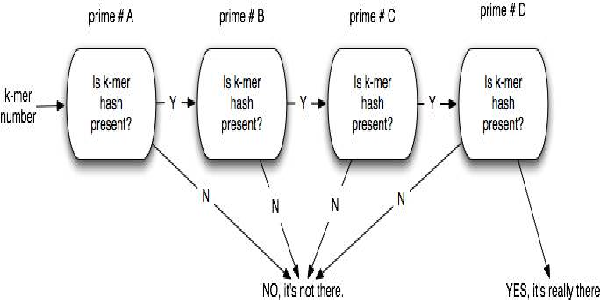
\includegraphics[width=5in]{figures/f1}}
\caption{Bloom filter.  @CTB also include a diagram of traversal algorithm.}
\end{figure}

We use a variation of the Bloom filter data structure to store k-mers
in memory. Rather than using multiple hash functions but only a single
hash table, we use a different hash table for each hash
function. Given a k-mer of interest, each table is queried for the
presence of a k-mer until the k-mer cannot be found in a hash
table. If each hash table contains the k-mer, then the k-mer may
be in the dataset. If any of the hash tables do not contain the
k-mer, then the data set definitely does not contain it. That is, there is a one-sided
error with false positives, but no false negatives. The many
calculable properties such as optimal number of hash functions that
can be determined for Bloom filters apply to our variation as well. To
demonstrate this, we stored 10,000 randomly generated 32-mers in our
data structure for a fixed amount of memory (50,000 bits). As we
varied the number of hash tables, we calculate the false positive
rate. We show in Figure X that the optimal number of hash
functions/tables is the same as the formula for a standard Bloom
filter. Thus, we can determine the overall false positive rate by
multiplying the occupancy for each hash table. Another advantage to
using a Bloom filter is that a linear increase in the amount of memory
used creates an exponential improvement in the false positive
rate. For example, ~4.78 bits per k-mer are needed for a false
positive rate of 10\% while ~6.22 bits per k-mer are need for a false
positive rate of
5\%. As with other hash-style data structures, Bloom filters have a
fast lookup time, which is O(h) when there are h hash tables to query
for k-mer presence.

\subsection{Using the Bloom filter as a k-mer graph.}
Having stored the k-mers into a Bloom filter, we are able to traverse
the corresponding k-mer graph. We let each k-mer be a vertex, where
the reverse complement of a k-mer is considered the same
vertex. Furthermore, we treat the graph as a simple graph as opposed
to a multigraph or digraph, which means that there can be no
self-loops or parallel edges between vertices/k-mers. Each k-mer can
have up to eight neighbors, with some exceptions: an alternating k-mer
(e.g. ATATA...) has seven neighbors and k-mers with each position
having the same base (e.g. AAAAA...) has six. In contrast to an exact
approach, there is a chance that a k-mer will be adjacent to a k-mer
that does not actually exist in the original dataset due to the false
positive rate from the Bloom filter. If this probability is too high,
it can be impossible to traverse given high enough K. For example, if
K is set to 32, no modern computer can explore each k-mer in a
reasonable period of time. Thus, if the false positive rate is too
high, graph traversal using a search algorithm such as breadth-first
search is infeasible.  (@CTB This deserves a better explanation, if
the point is to prepare the reader for the percolation discussion.)

Note that the primary data structure is constant in its memory usage,
so only ancillary information (list of nodes already visited, or
waypoints in the graph) consumes additional memory.

\subsection{Effect of false positives on local graph structure}

%% This representation has a one-sided error that we can measure and
%% predict in terms of its impact on graph properties.  Link degradation
%% to percolation here.

\begin{figure}
\center{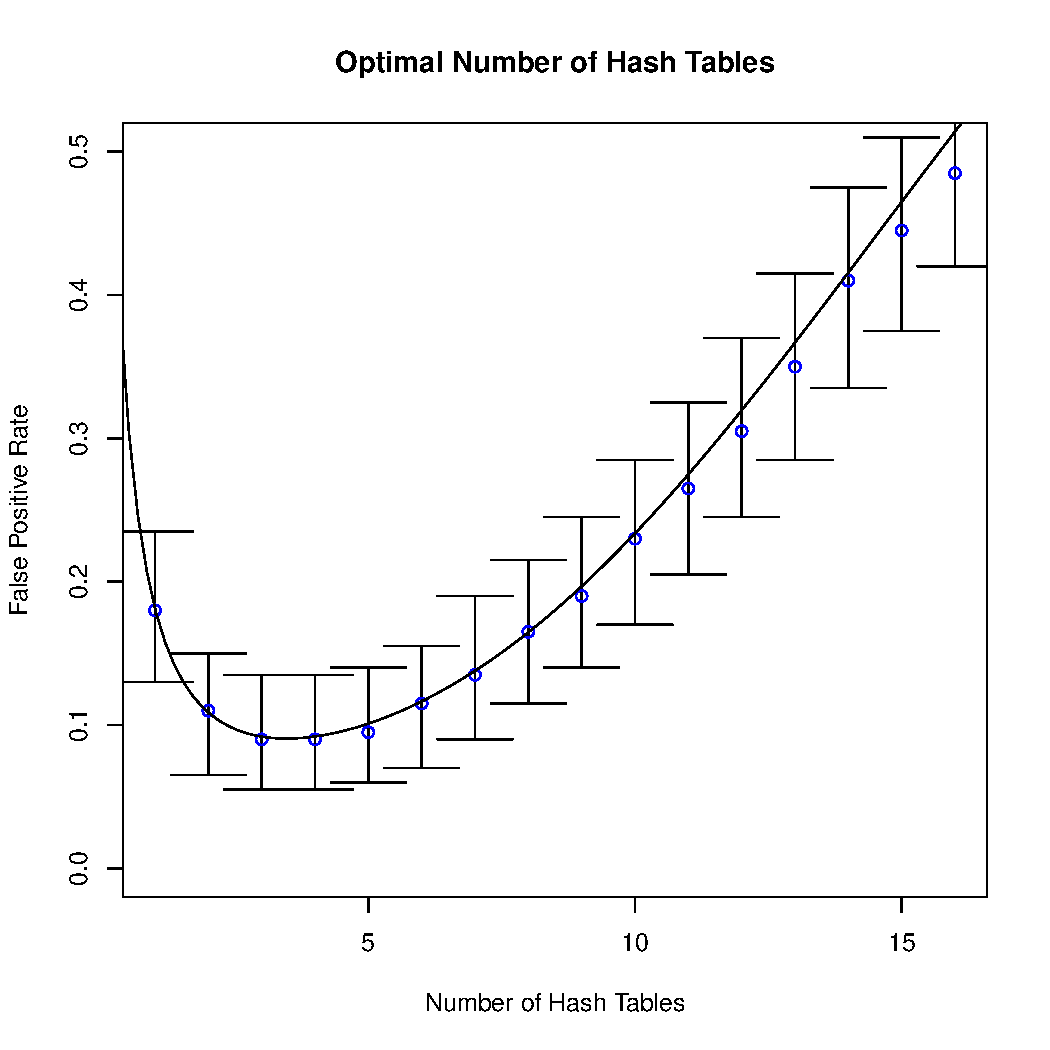
\includegraphics[width=5in]{figures/optht}}
\caption{There is a minimum false positive rate for a given amount of memory
and amount of data, set by the number of hash tables.}
\end{figure}

\subsection{Percolation theory in k-mer graphs.}

(Motivation? @CTB) While the local structure degrades smoothly with the
false positive rate, we want to know how global connectivity degrades.
We also want to know how easy it is to detect this degradation, i.e. at
what FP rate do we systematically buy ourselves trouble?

As the false positive rate increases, there appears to be a sudden
transition between the point where graph traversal is possible and
when it is not. This rapid change resembles a phase transition in the
field of physics, which ultimately relates to percolation theory (@CTB
isn't this the other way around? percolation to phase transition?). As
long as the false positive rate is below the percolation threshold (in
the subcritical phase), it is possible to traverse the graph. If the
false positive rate is above (in the supercritical phase), then graph
traversal is infeasible. We randomly inserted 31-mers into Bloom
filters with different false positive rates and calculated the average
cluster size for each. Figure X demonstrates that the average cluster
size rapidly increases as the percolation threshold is approached,
which appears to be at a FP rate between 0.17 and 0.18 for k=31. This
graph also suggests that up to the percolation threshold, graph
partitioning is possible but becomes slower as the threshold is
approached.

\subsection{Large-scale graph structure retained to percolation threshold.} We
randomly generated a 1,000bp sequence and added the first 31-mer to
the end to create a circular chromosome with 1,000 31-mers. Then,
using four different false positive rates (fpr=0.01, 0.05, 0.10, and
0.15), we explored the graph using breadth-first search beginning at
the first 31-mer. We then used the graph
layout package graphviz for visualization. The graphs demonstrate how
the local graph structure begins to change while the original circular
graph remains intact with no erroneous paths between k-mers that are
truly present in the originally generated sequence. Because the k-mer
space is so large for large enough K, a high false positive rate below
the percolation threshold is still unlikely to connect components
together erroneously. We further note that when the false positive
rate is above the percolation threshold, the resulting graph would be
impossible to visualize for large values of k.

@CTB would like graph of change in longest shortest path between all
pairs of k-mers, to illustrate the global graph structure does not change.

\subsection{Sequencing errors eclipse errors from graph representation.} One
important consideration when determining the usefulness of our k-mer
graph representation is how it compares to errors from massively
parallel sequencers such as Illumina. In de Bruijn graph-based
assemblers, sequencing errors add to the graph complexity and make it
more difficult to find high-quality paths for generating long,
accurate contigs[assembly review paper?]. Since our approach generates
a different type of error, we aim to show that for a reasonable false
positive rate, sequencing errors dominate the graph complexity
issue. We used an E. coli dataset provided by Illumina to compare
various graph invariants between the Illumina dataset, an exact
representation of the genome, and various inexact representations with
different false positive rates.  (@CTB repeat with newer E. coli data.)

\begin{figure}
\center{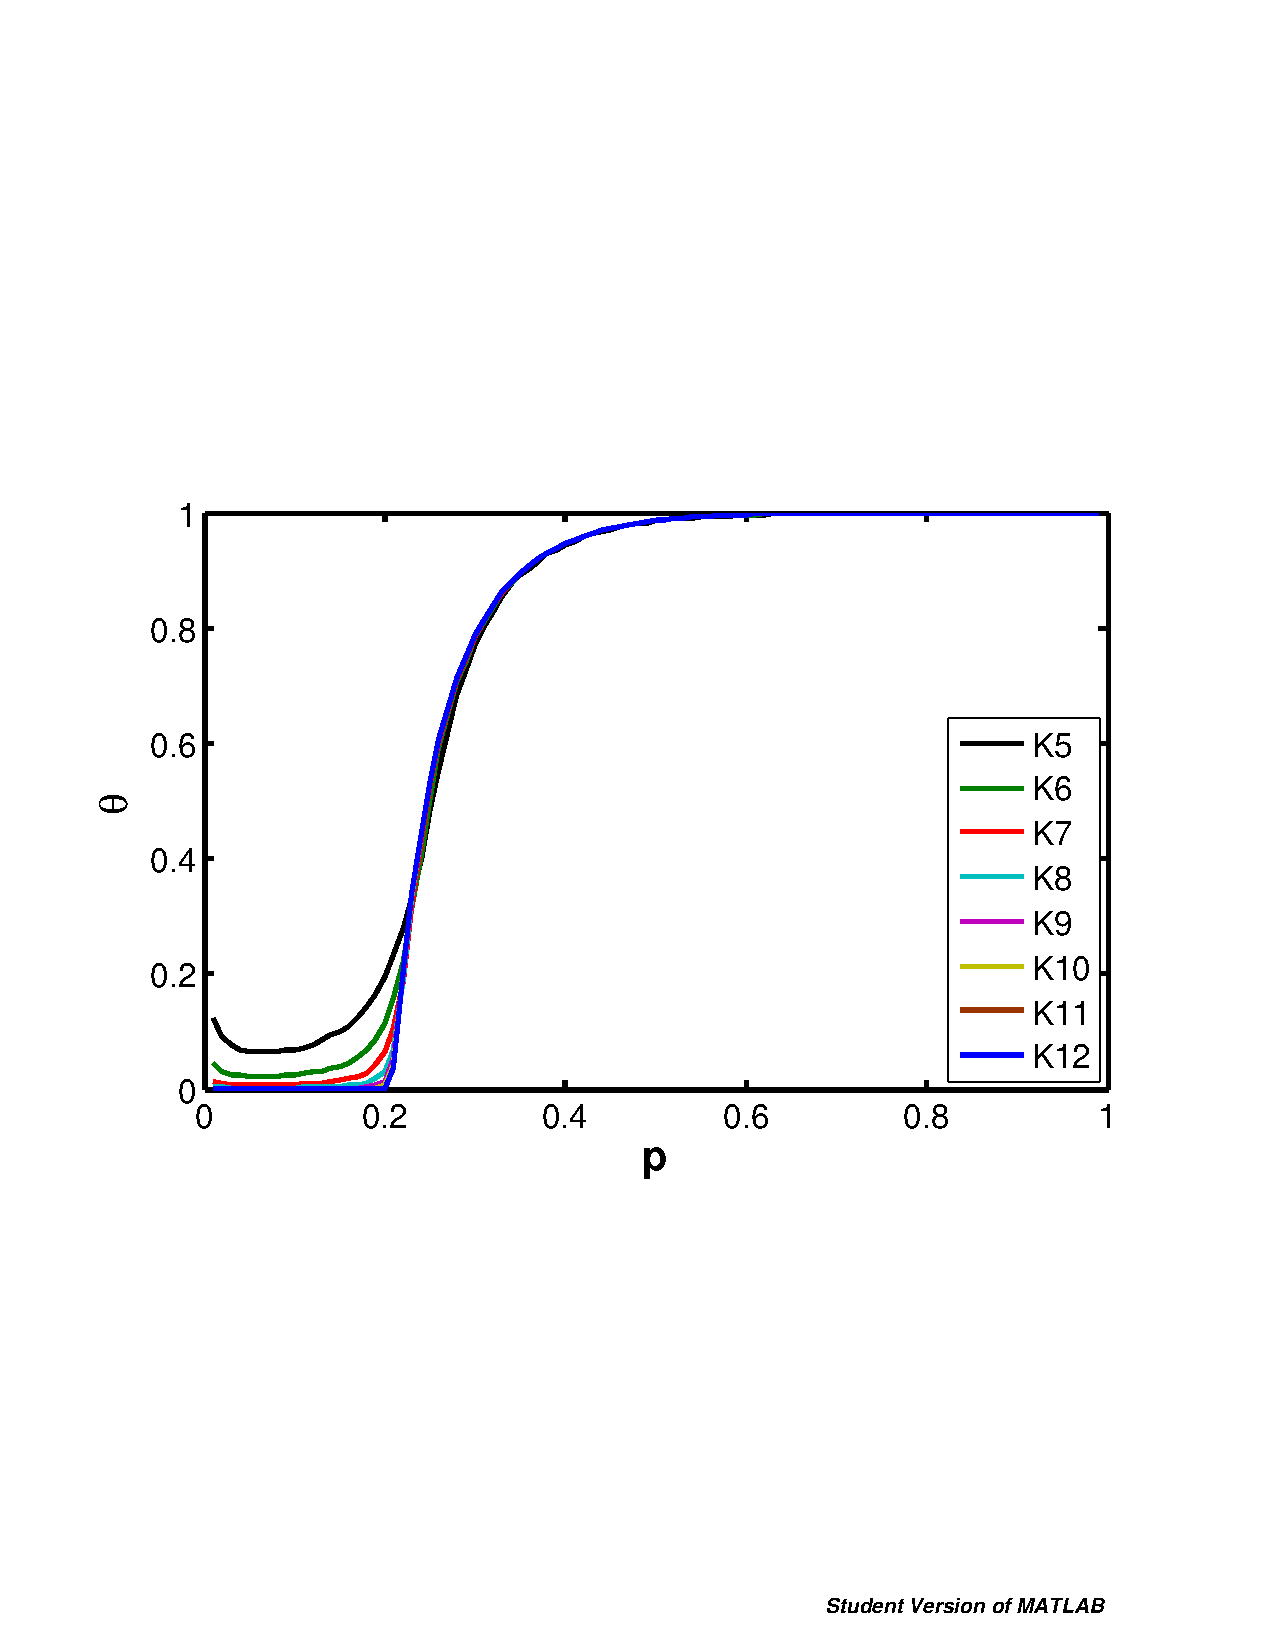
\includegraphics[width=5in]{percolation_K5_to_K12_withLegend}}

\caption{K independence, relative size of the largest connected component
$\theta$ for kMer occupancy p (0.0 to 1.0) of various de Bruijn graphs of
different sizes K (5 to 12 see legend), showing the independence of the
percolation threshold ($\theta = 0.5$) from K.
For each datapoint p 1000 random samples were generated keeping the std error
for each datapoint under 0.0047 while the mean std error for all data points is
$< \approx 0.0002$ (data not shown).}
\end{figure}

\begin{figure}
\center{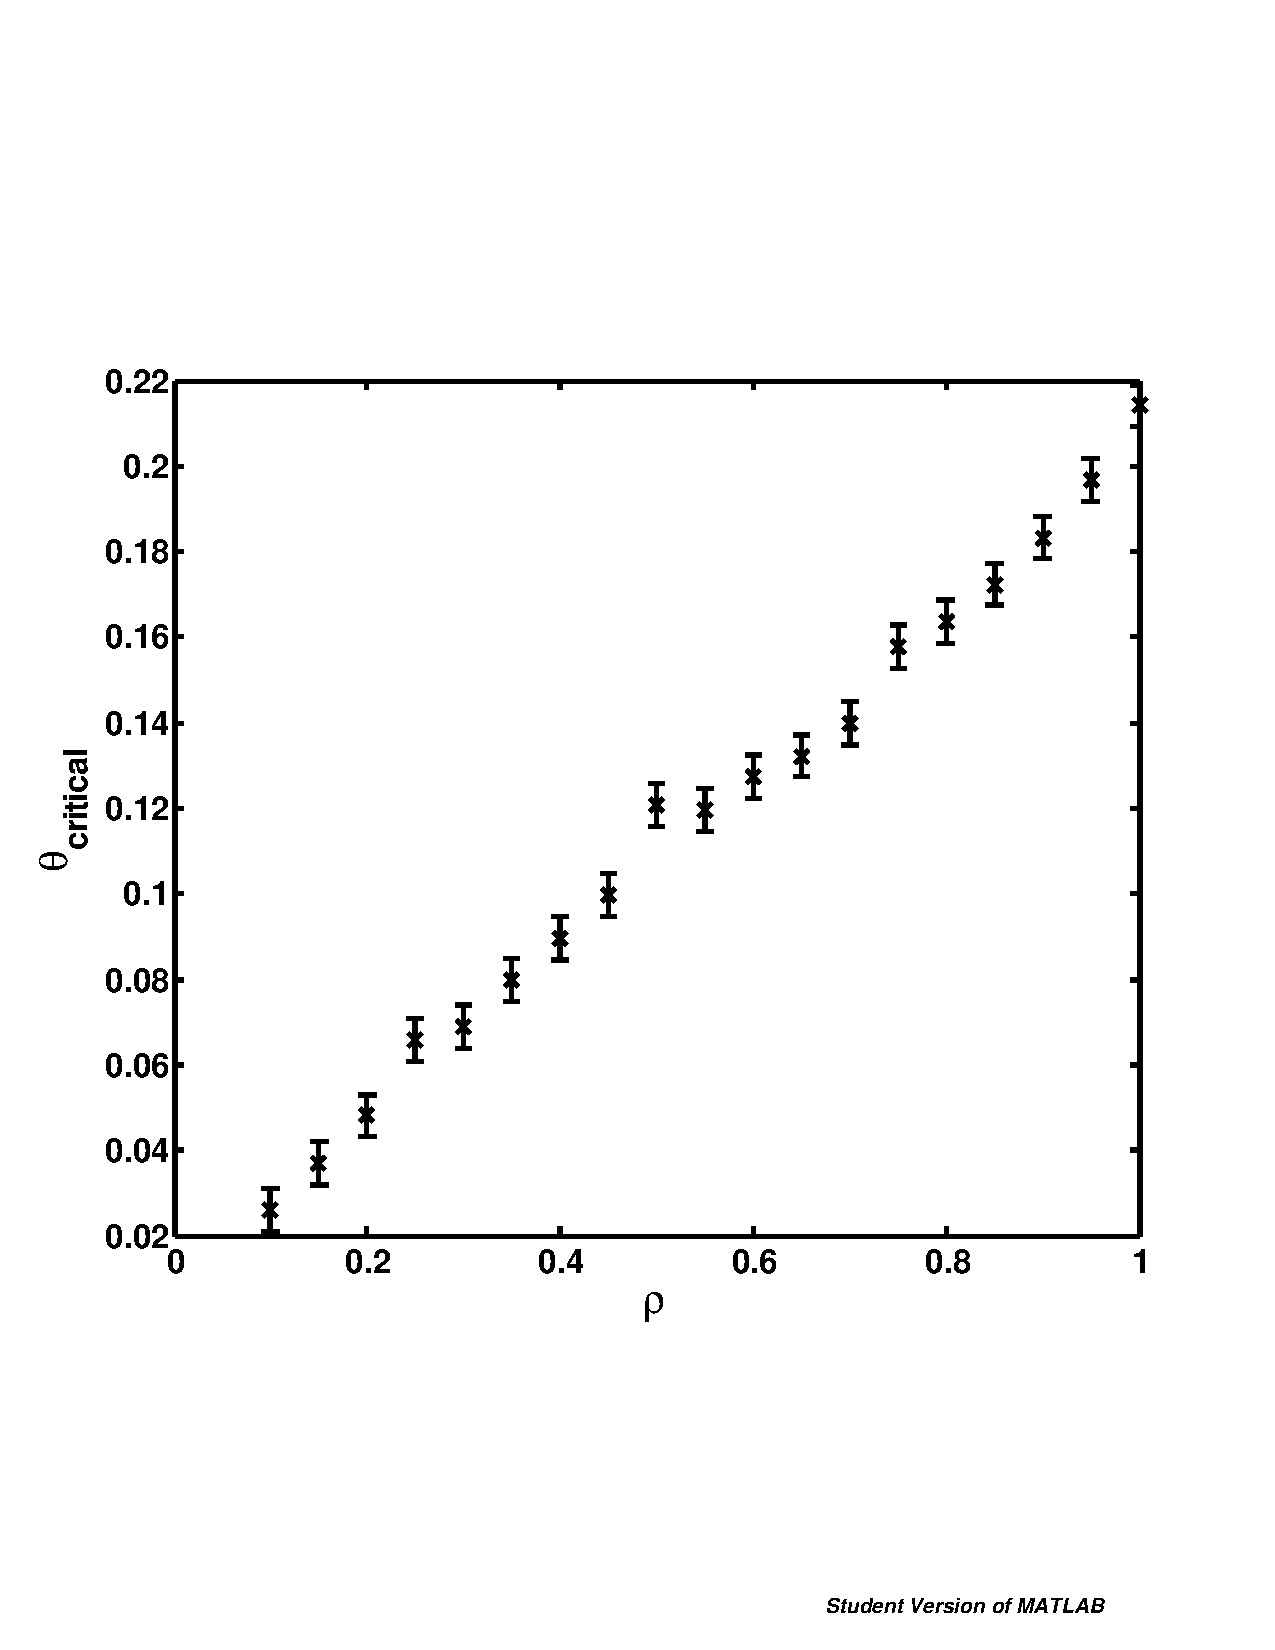
\includegraphics[width=3in]{memoryFraction_vs_percolationThreshold}}
\caption{The critical point for percolation is linearly related to the
  compression factor of the graph representation.  (@CTB Y axis should end at 0.)
This figure shows
  the interpolated critical percolation threshold dependence on the
  memory used for the Bloom filter. $\rho$ is the fraction of
  maximally required memory ($4^{12}$ bits) for a de Bruijn graph with
  K=12. We reduced the memory allowed $\rho$ from 1.0 to 0.1 (x
  axis). The critical percolation threshold $\theta_{\rm critical}$
  was linearly interpolated (at the critical point $\theta=0.5$ the
  slope is infinite allowing for this). The std deviation is given for
  each interpolation. This plot shows a linear relation between
  allowed memory and expected percolation threshold assuming random
  data. We can fit the following function to this plot: $\theta_{\rm
    critical} = 0.209 \rho + 0.0052$ describing the fraction of memory
  where random data would percolate.  {\bf CTB: this linear result is
    what you'd expect if the slope of the approach to percolation
    across increased occupancy is exponential, given the logarithimic
    false positive rate wrt memory?}}

\end{figure}

%% \subsection{This can usefully be applied to assembly graphs}

%% We can use this to look at local assembly graphs usefully.

\begin{figure}
\center{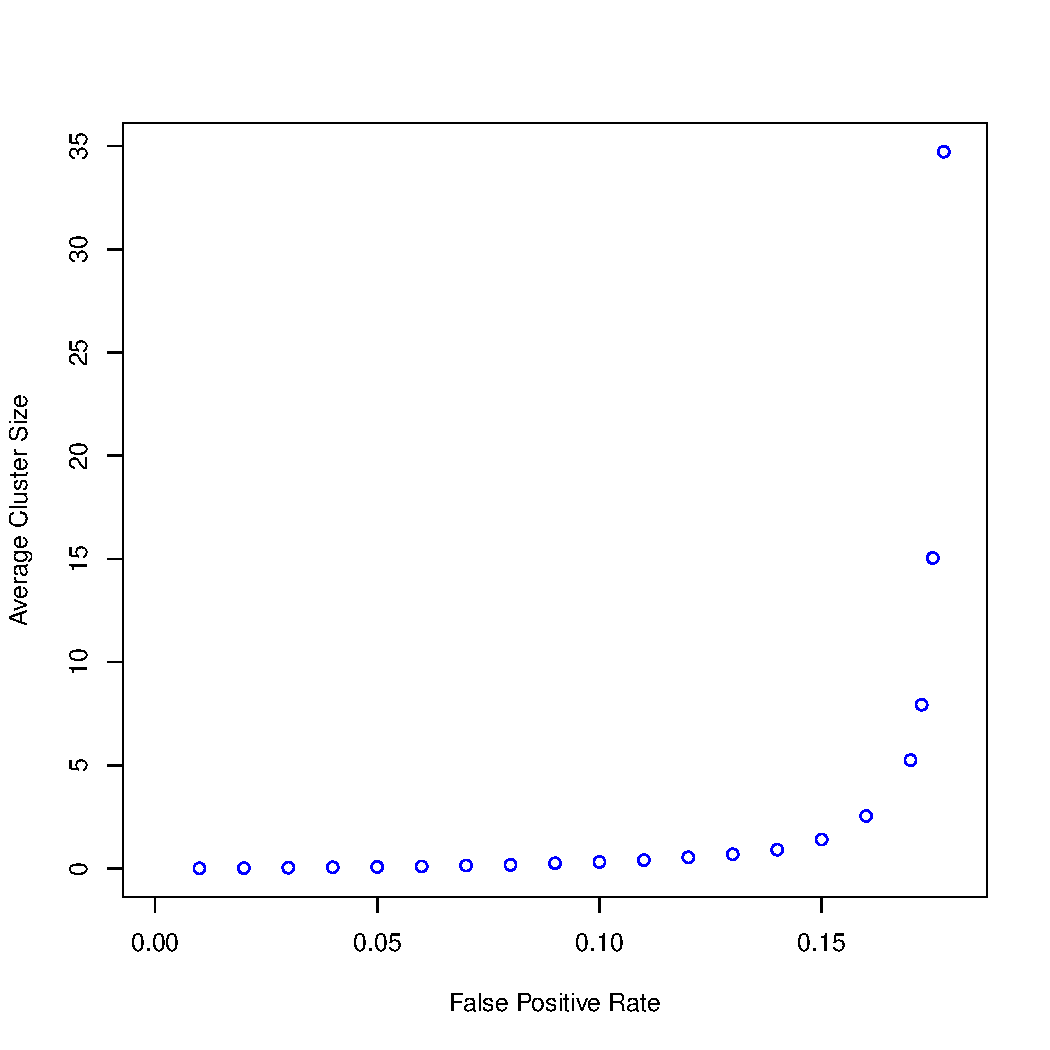
\includegraphics[width=5in]{k31}}
\caption{Approach to critical percolation limit. {\bf Is this an
    exponential?  Or what?  Might be too sharp for that, but what
    would the functional form be? Can we fit?  Do we know the constants?}}
\end{figure}

\begin{figure}
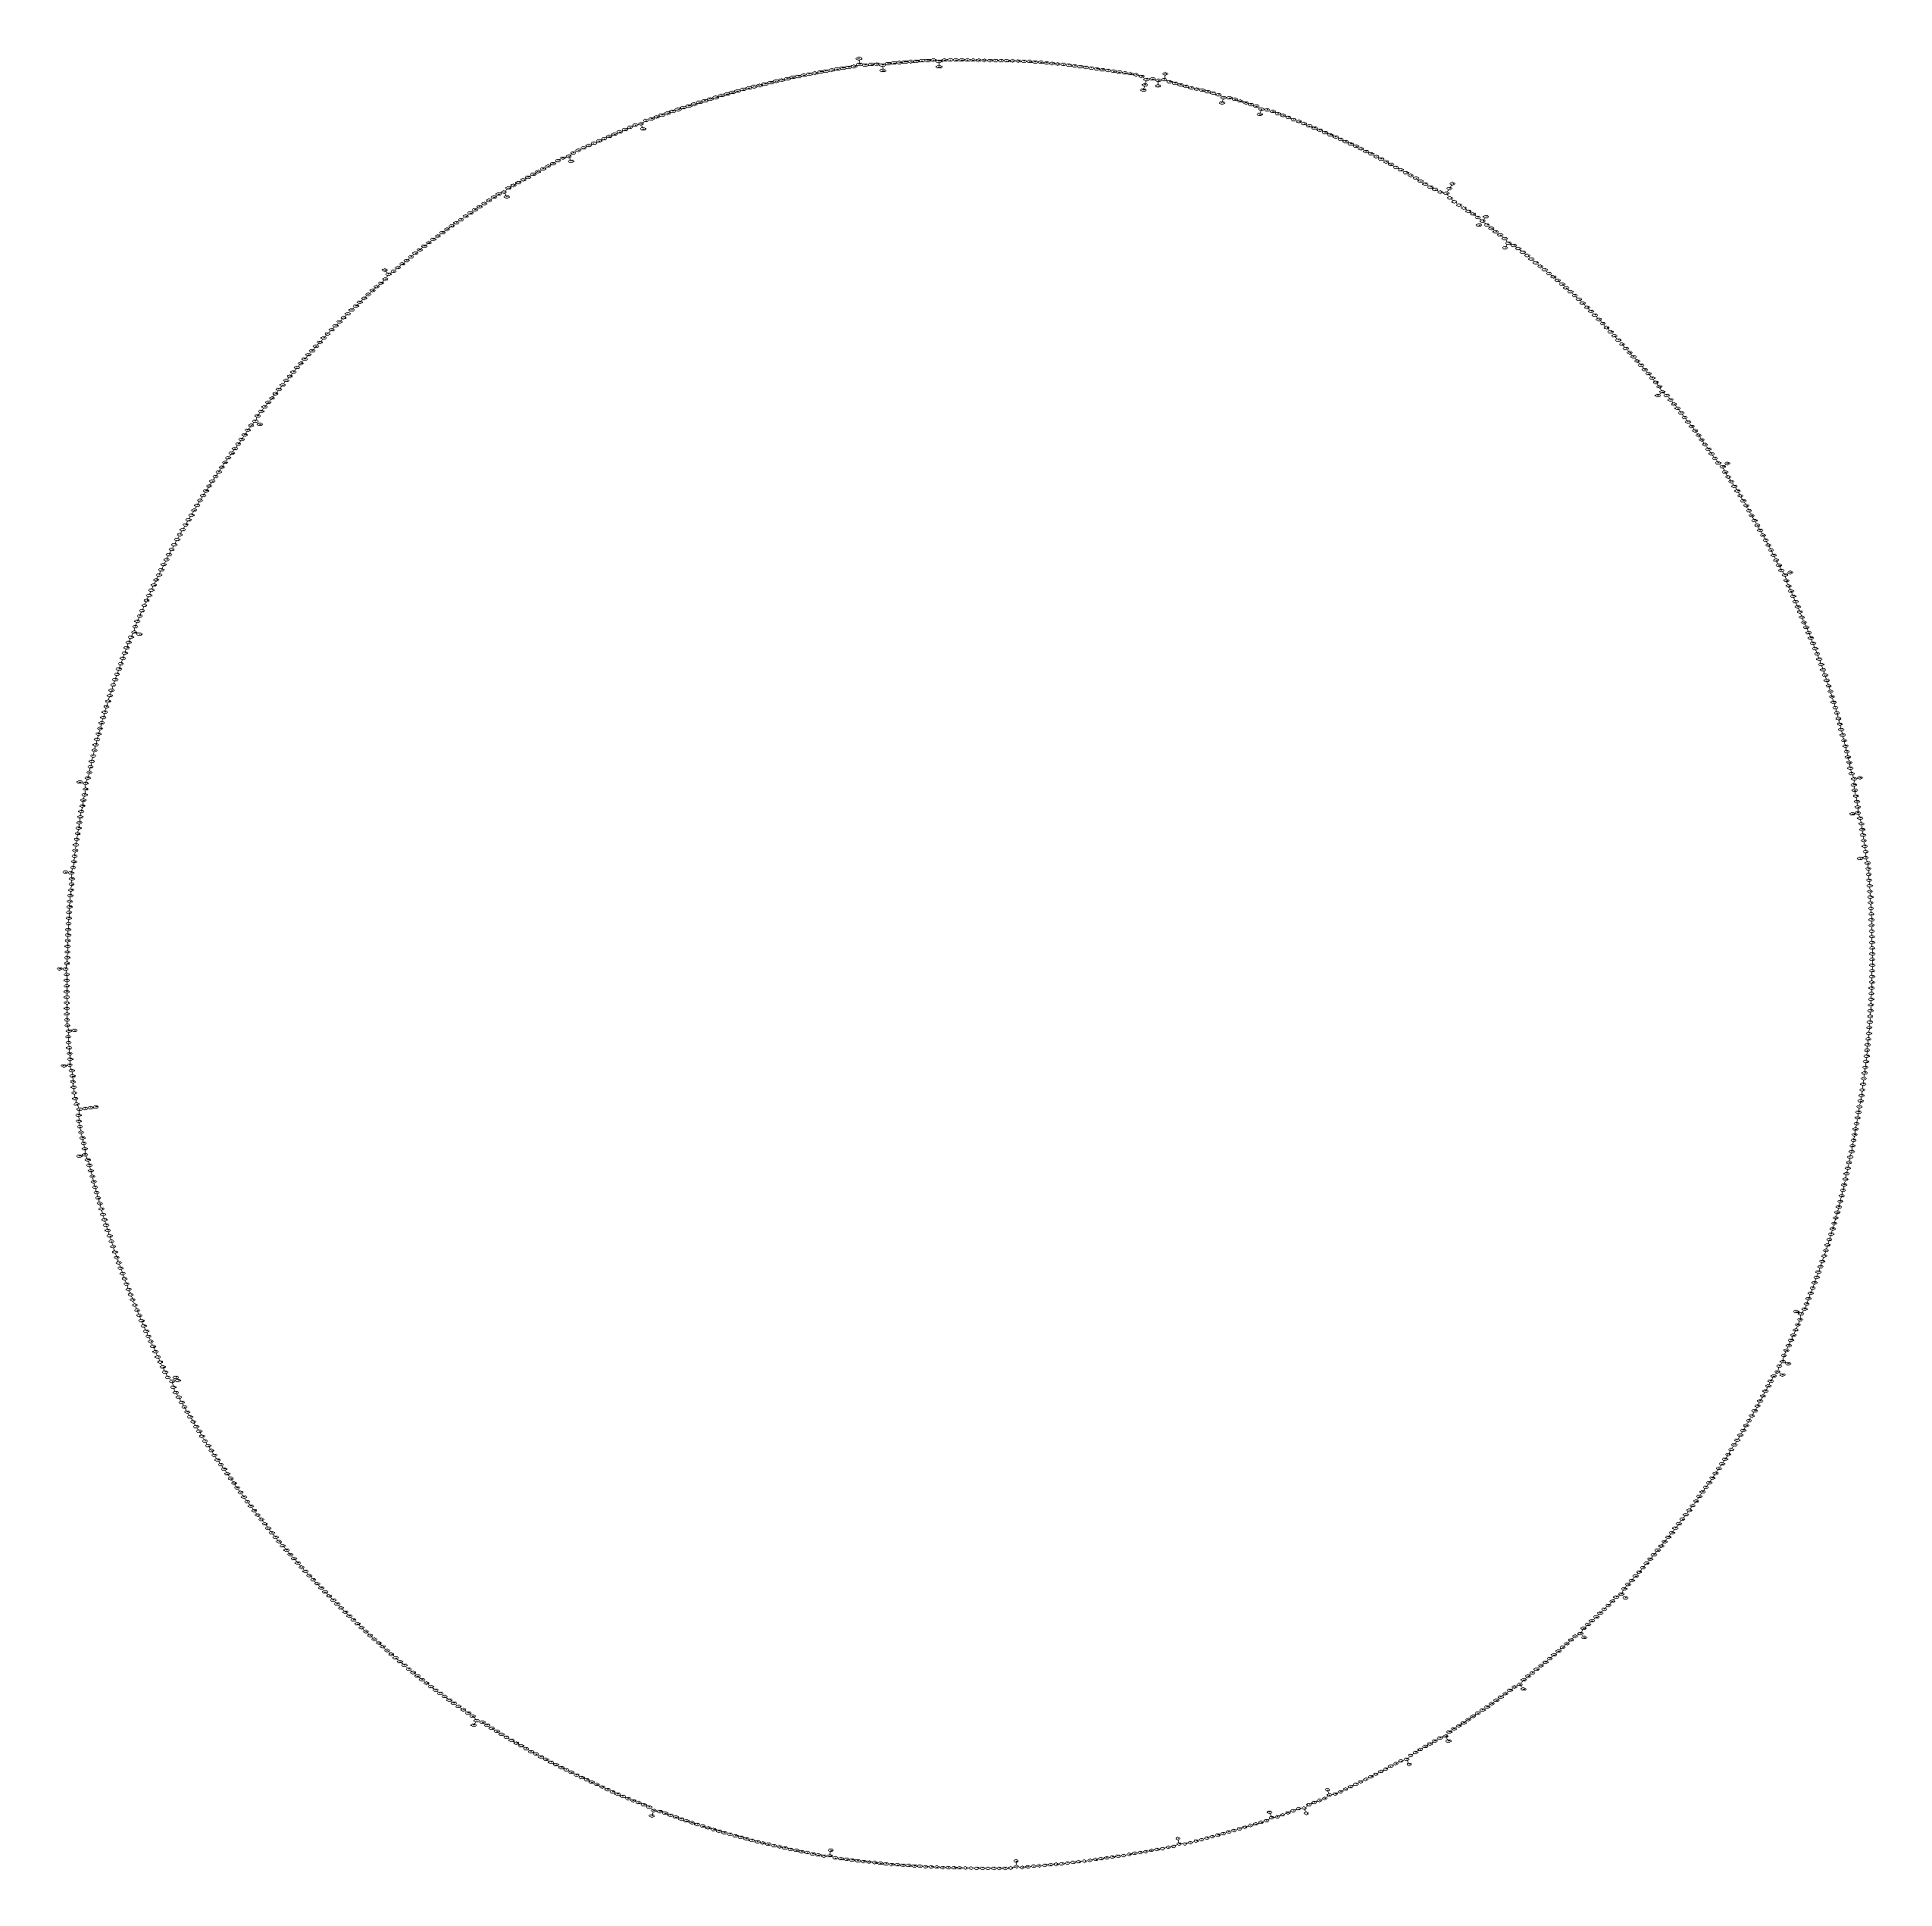
\includegraphics[width=3in]{figures/f3b001}
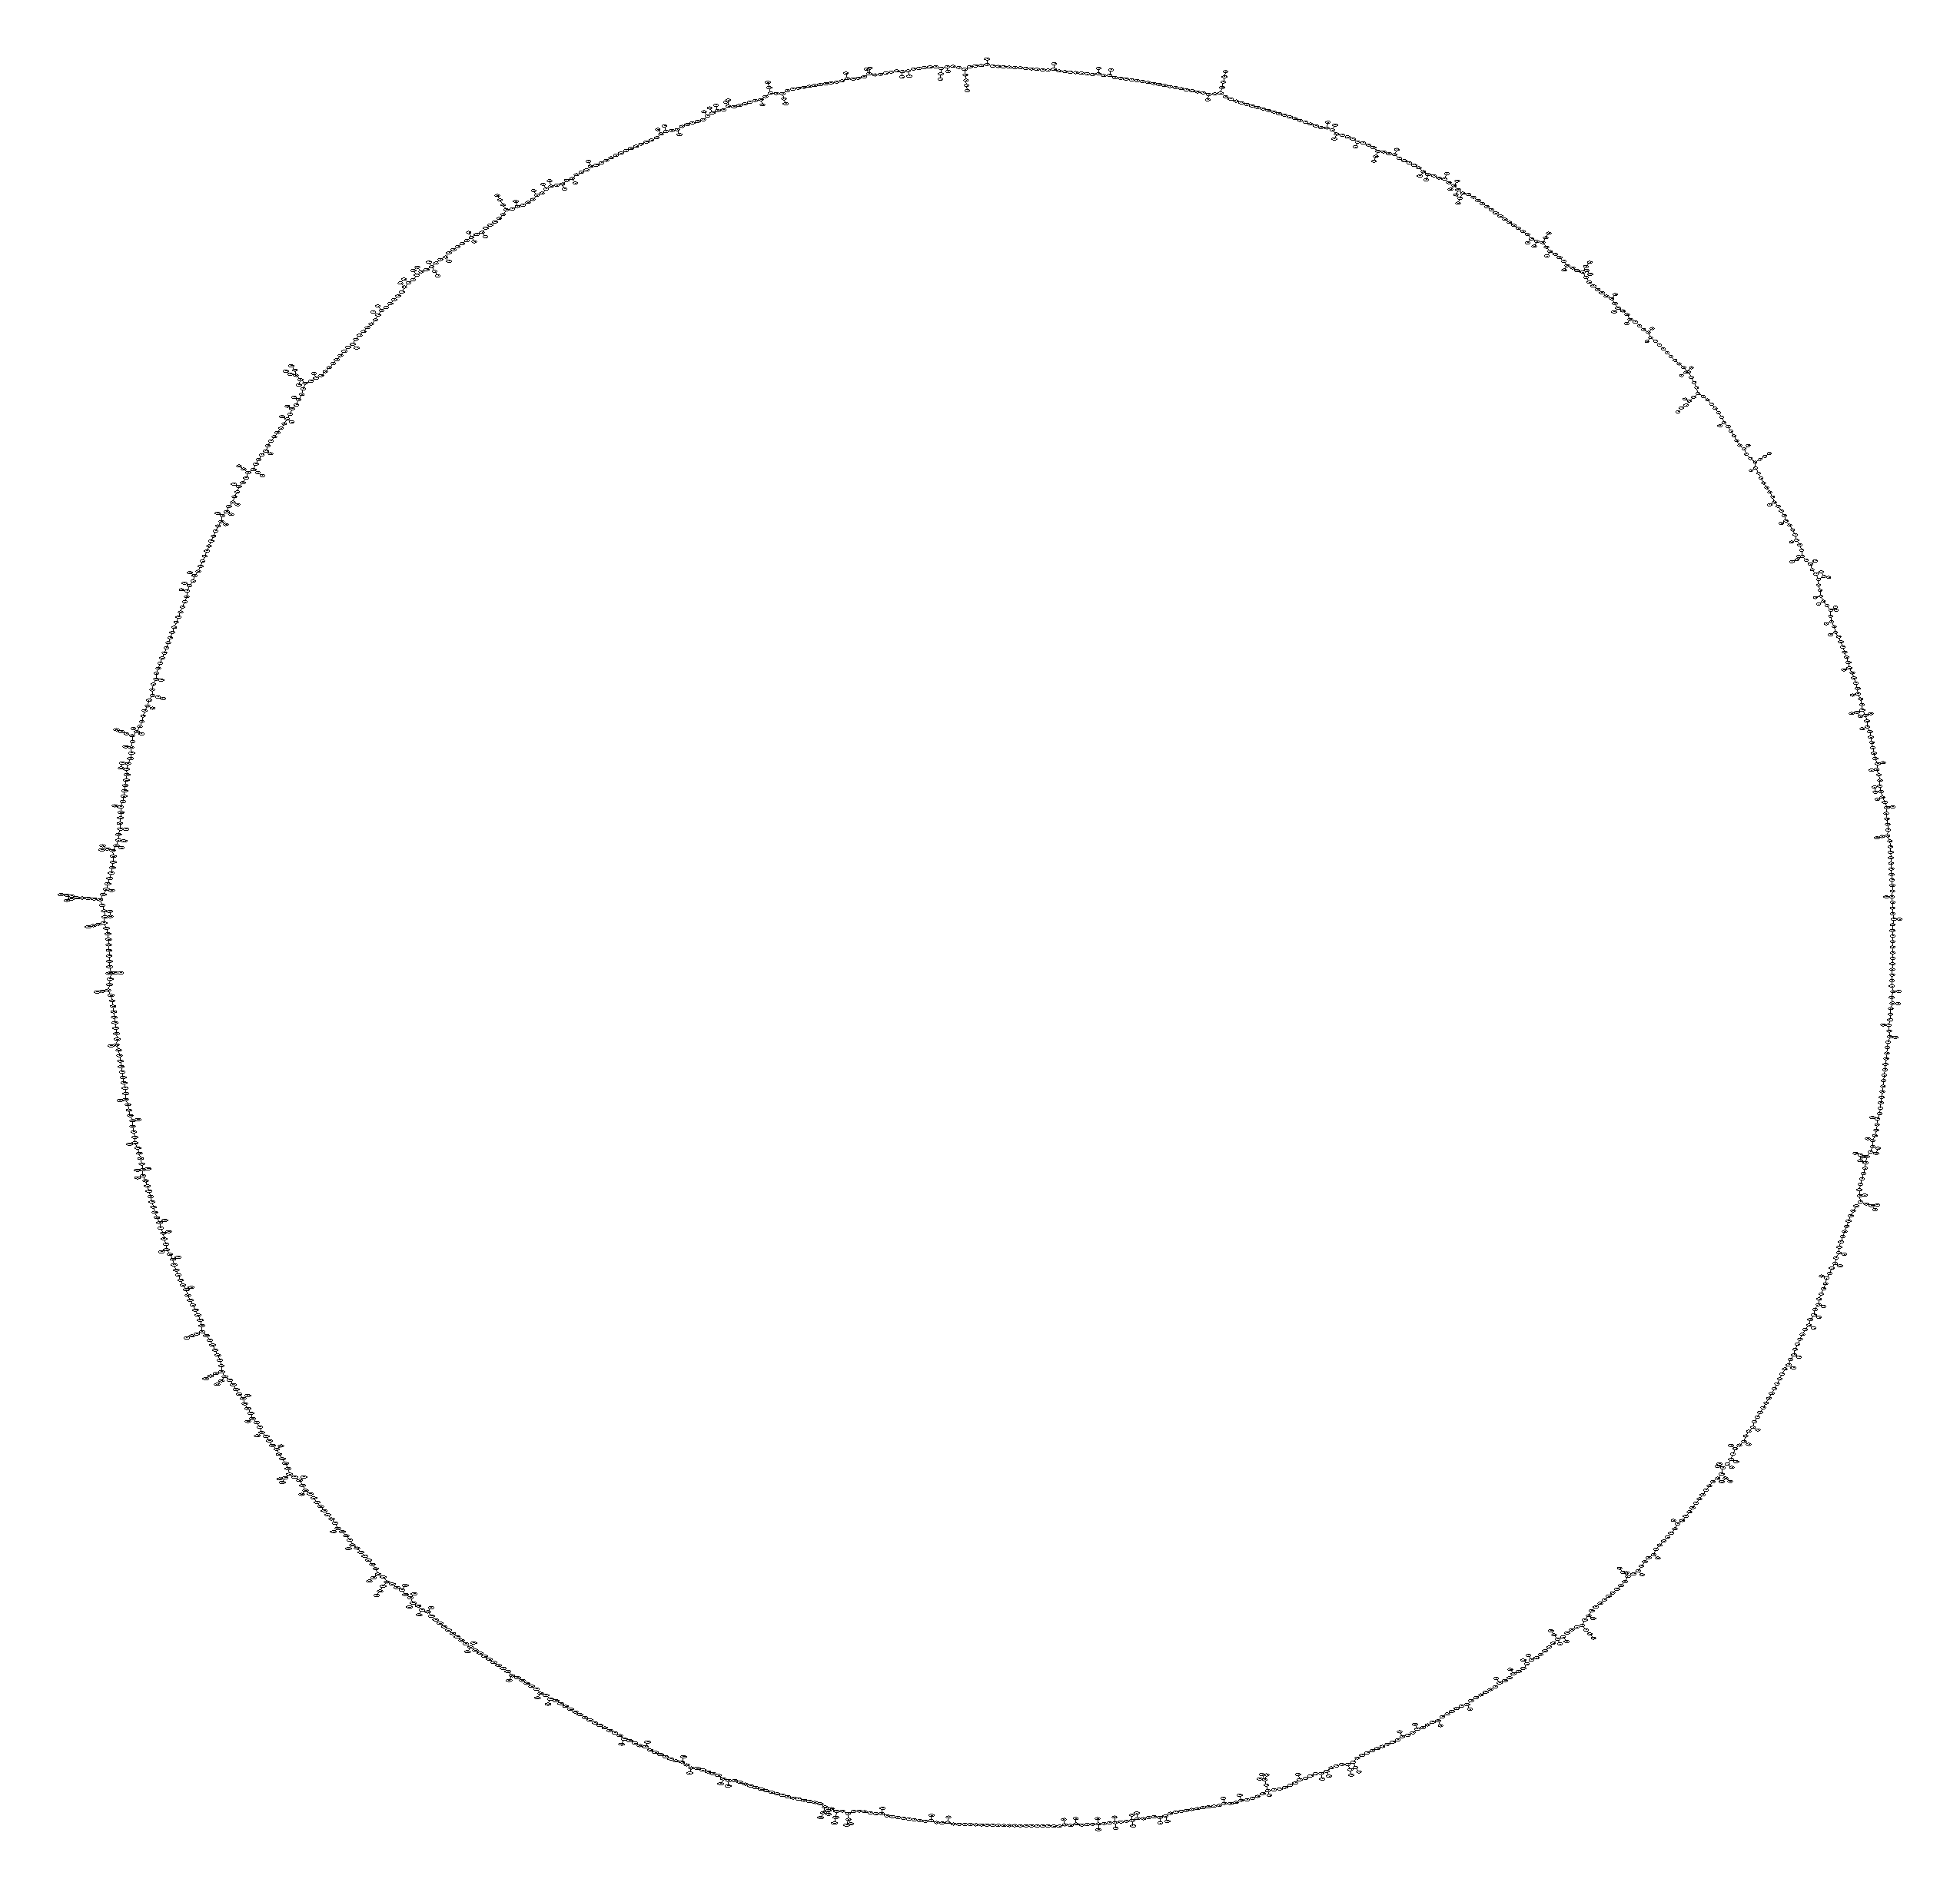
\includegraphics[width=3in]{figures/f3b005}\\
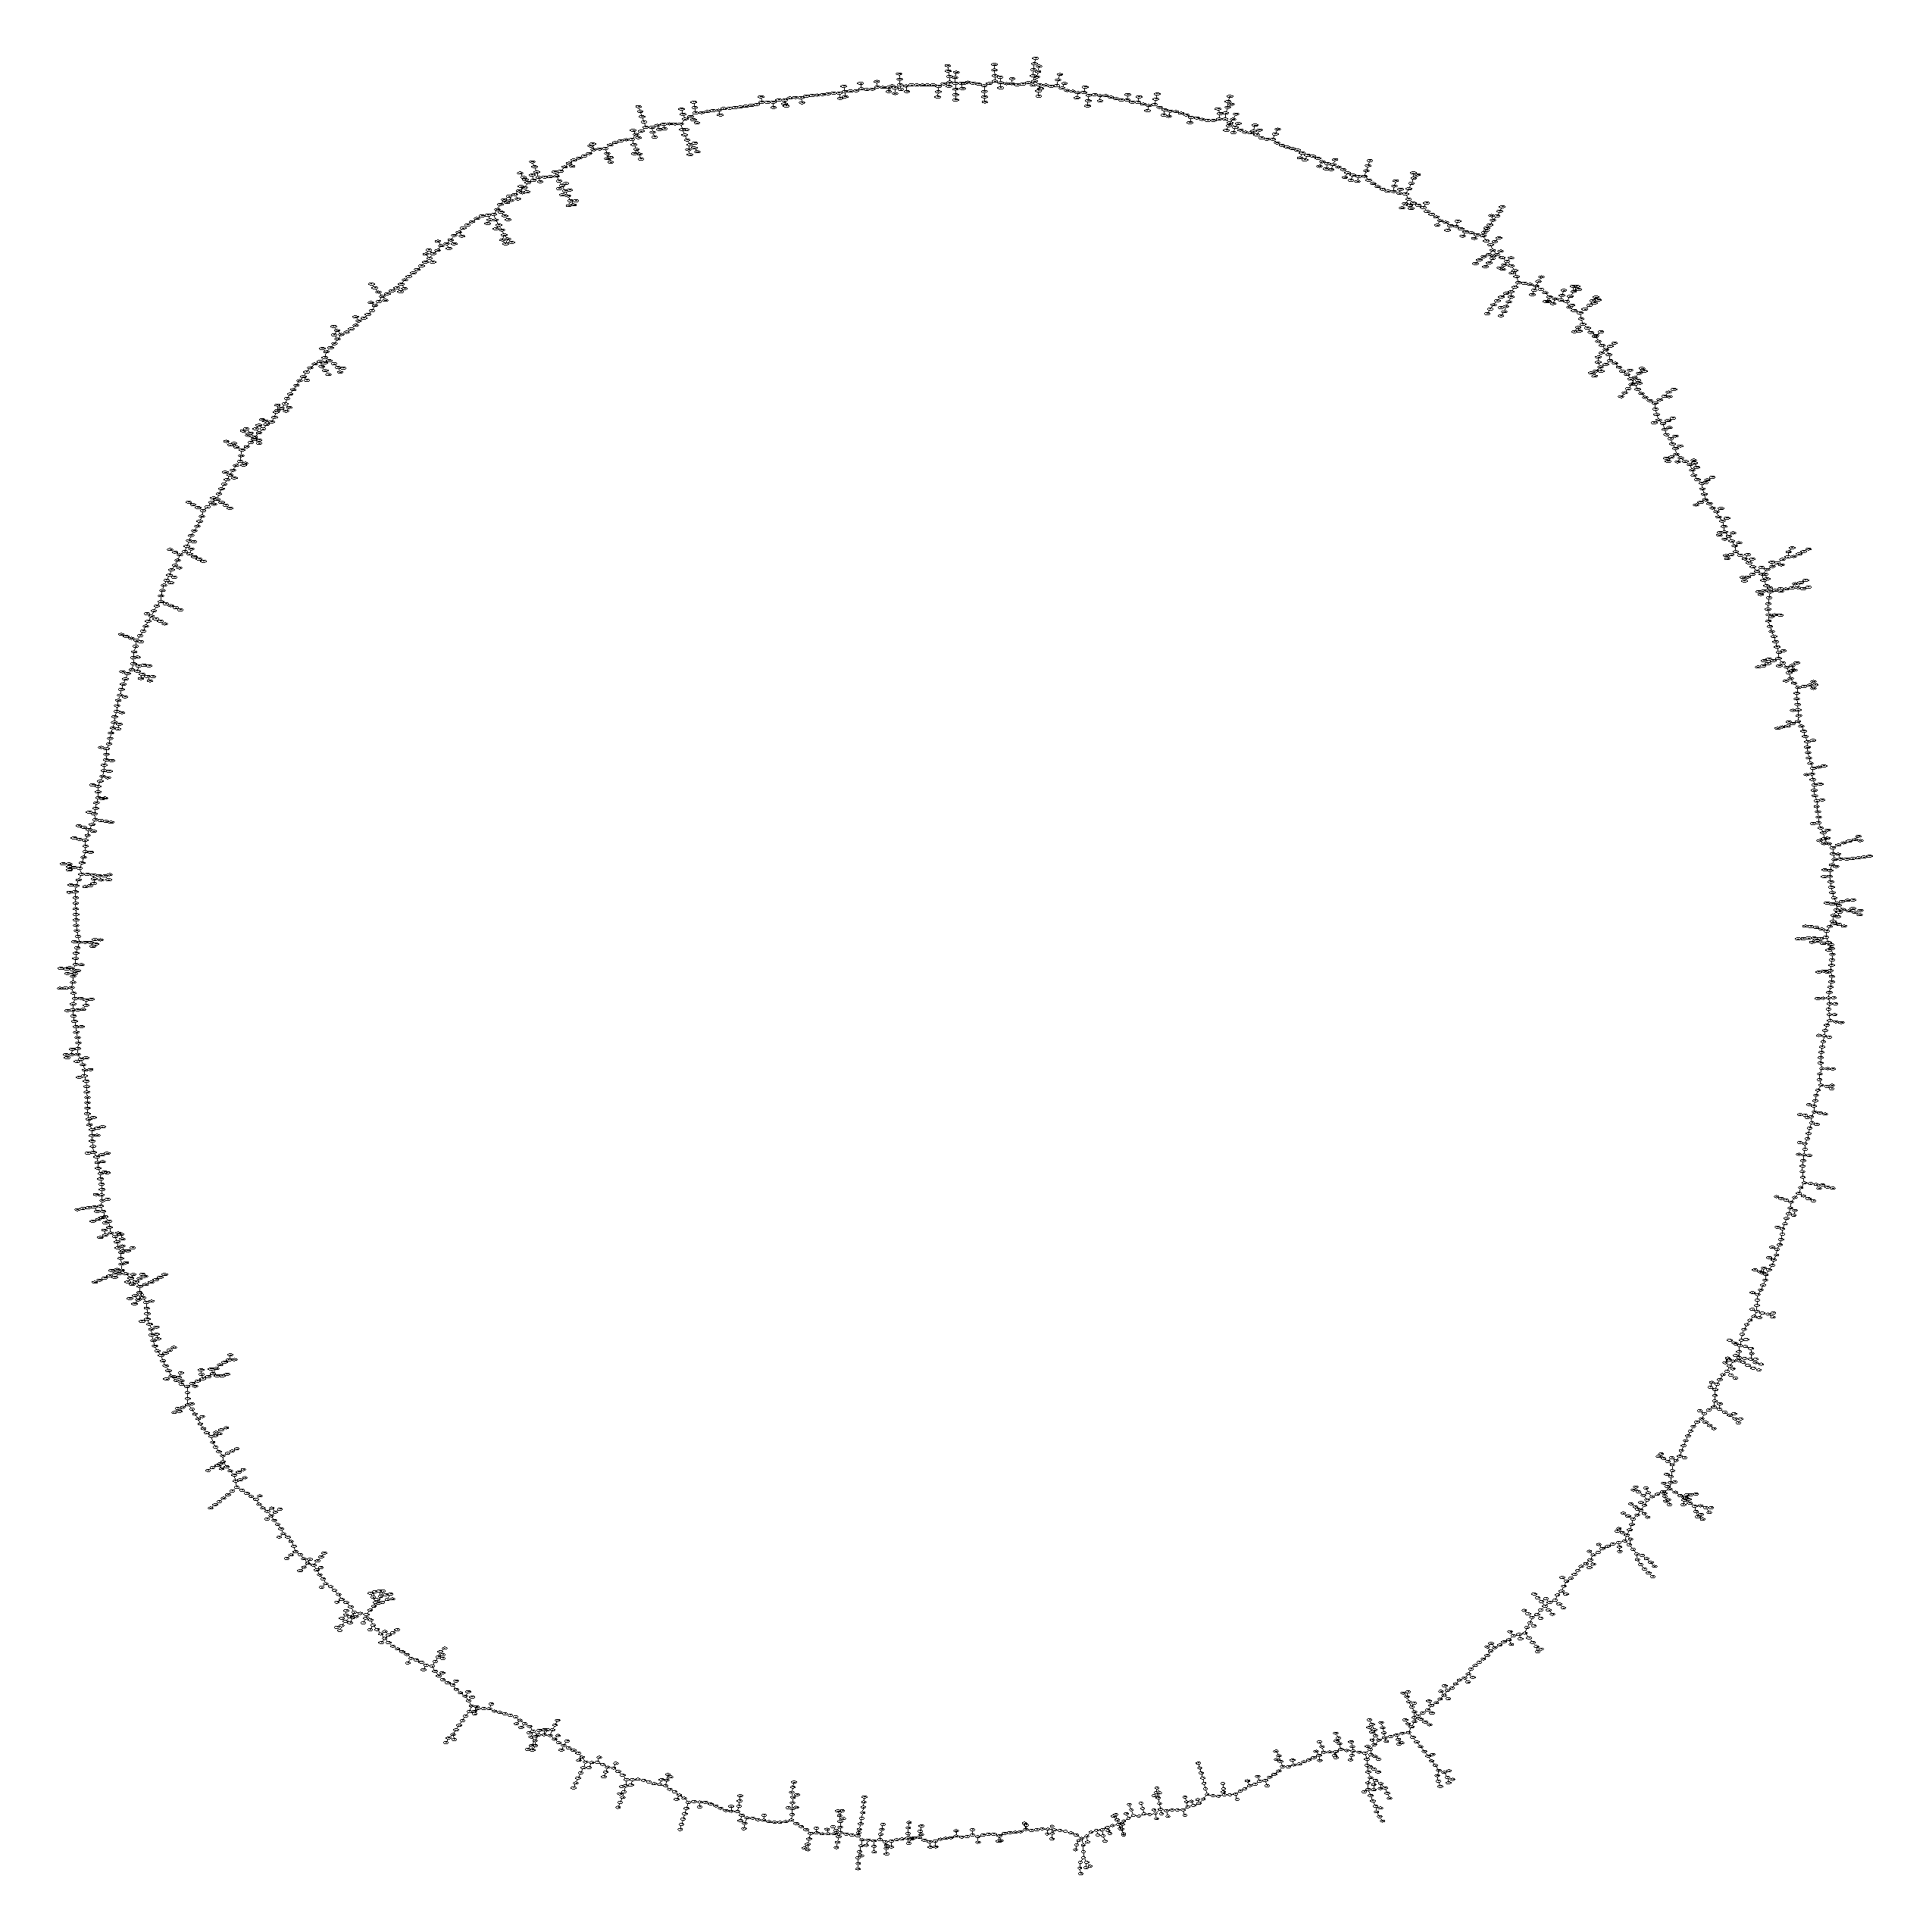
\includegraphics[width=3in]{figures/f3b010}
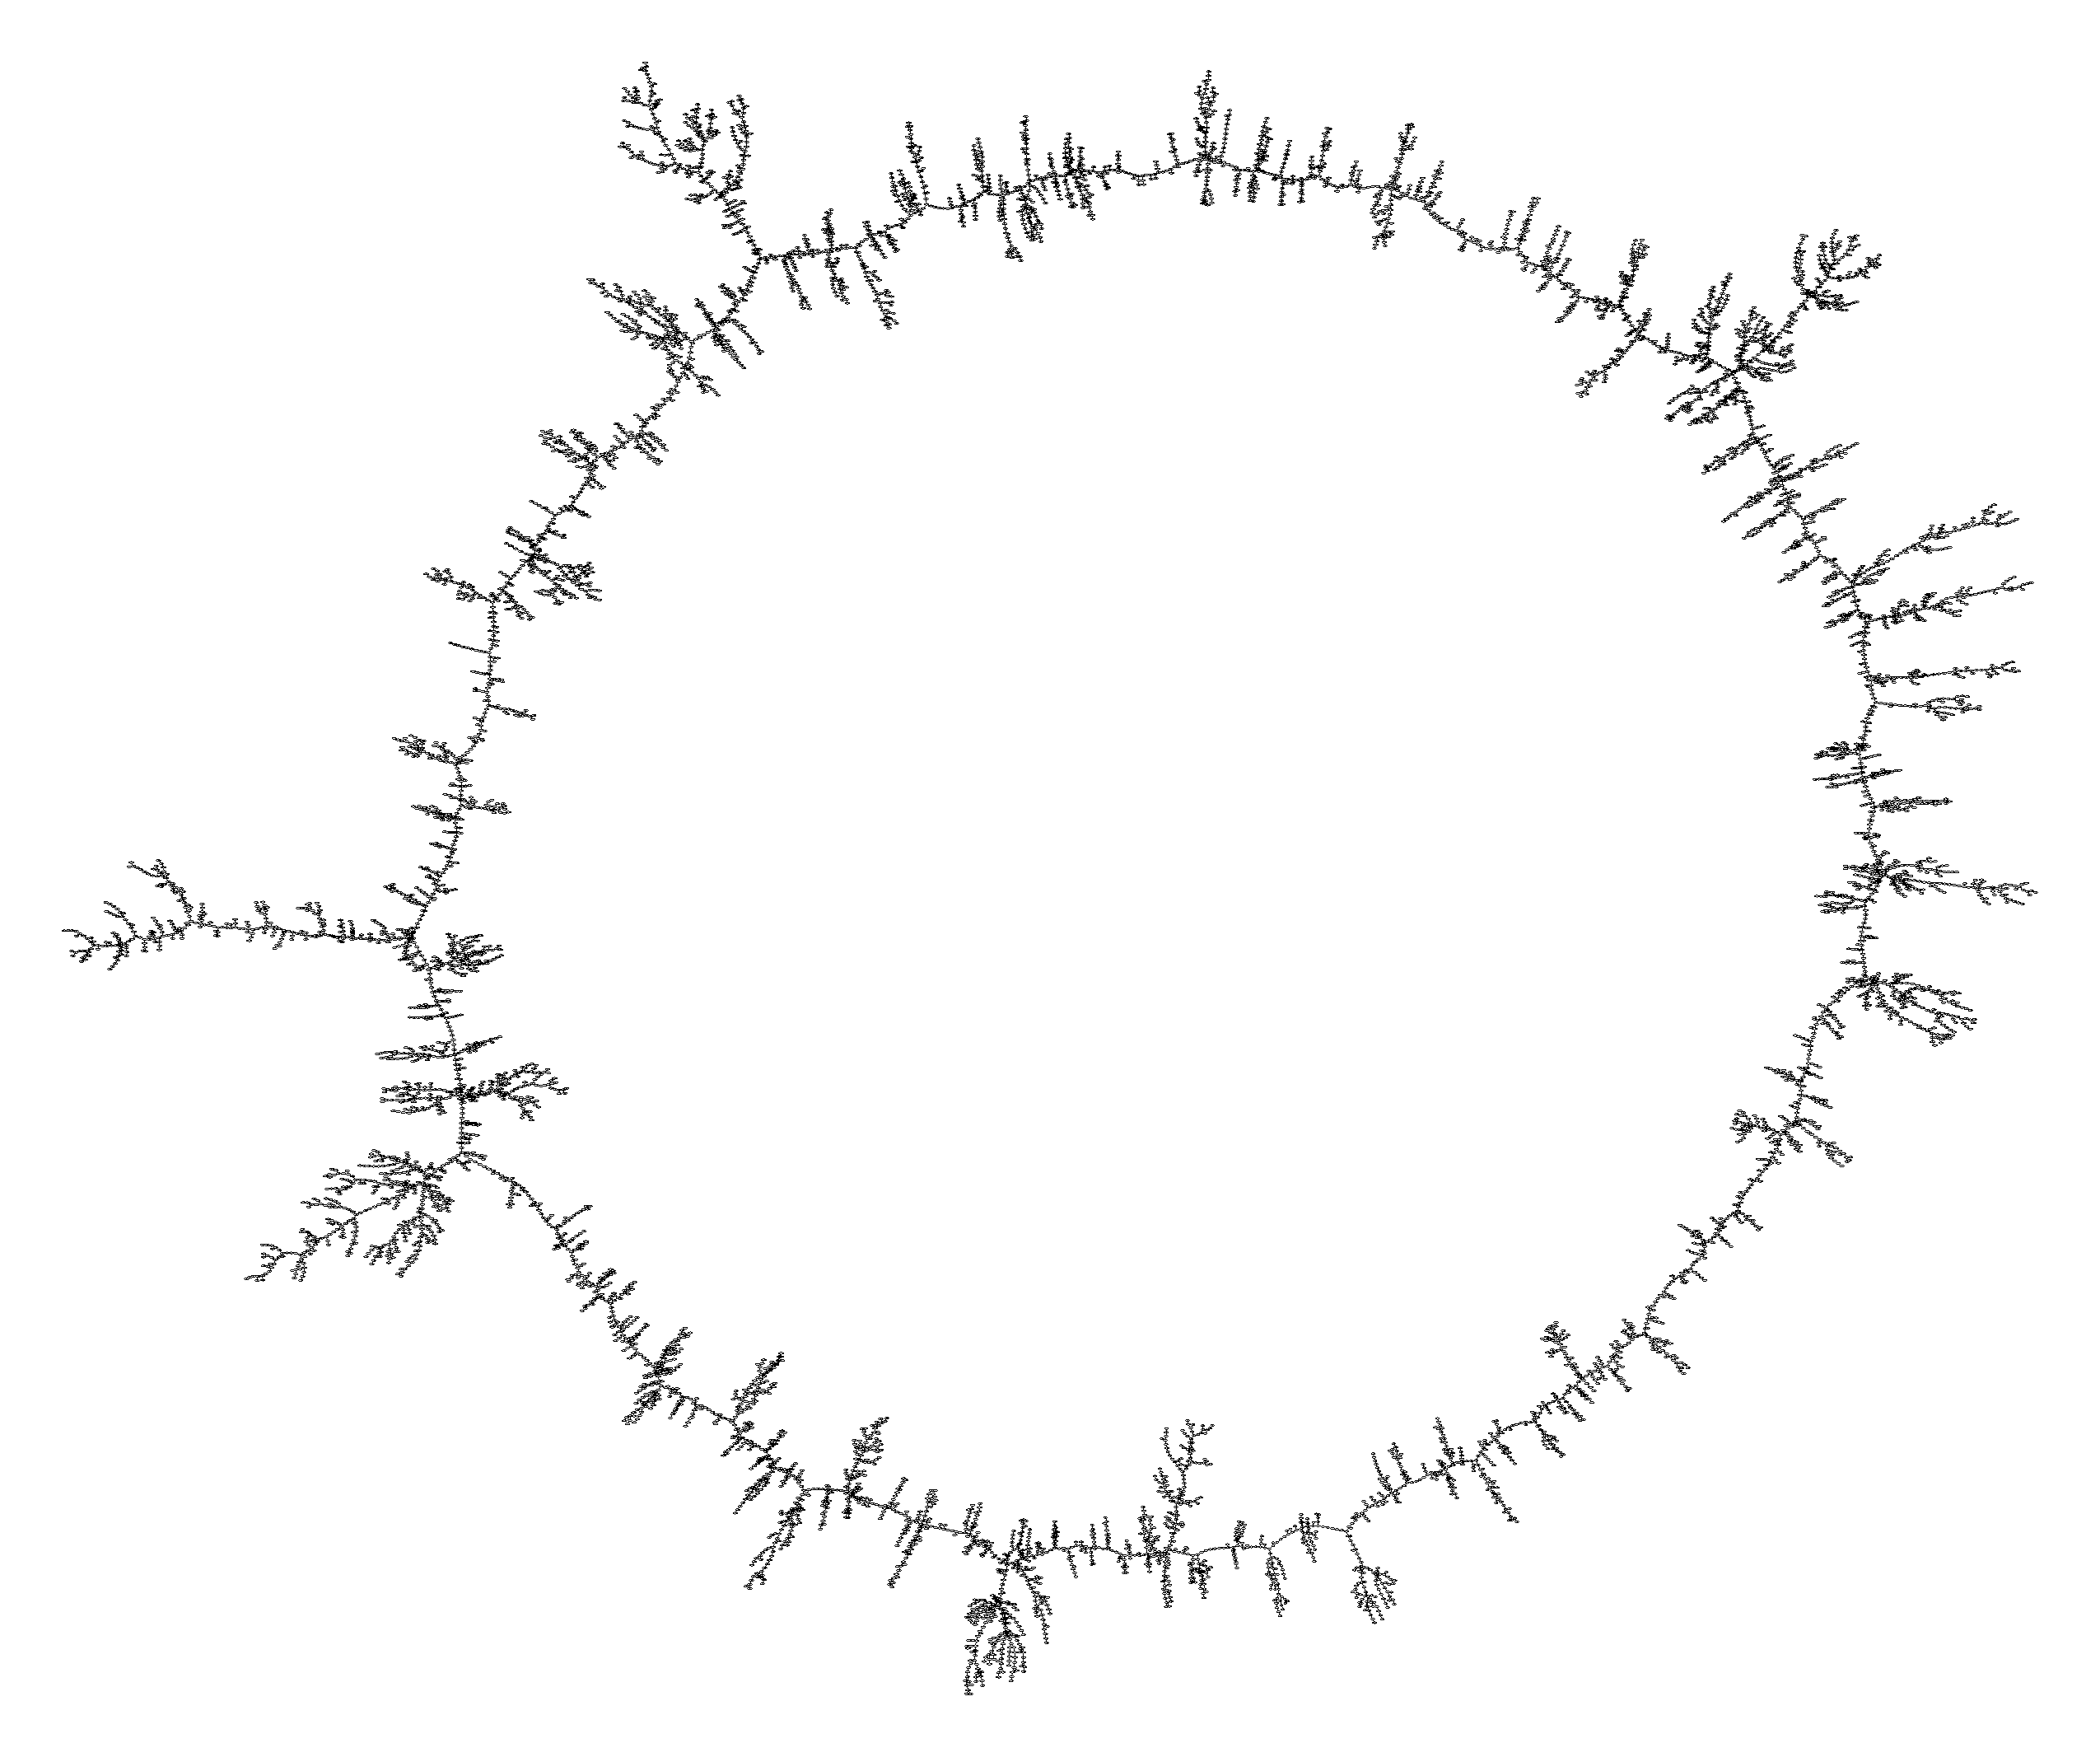
\includegraphics[width=3in]{figures/f3b015}
\caption{Decreasing fidelity of graph structure with false positive rate.
{\bf CTB: This should be our first figure, I think!}}
\end{figure}

\section{Discussion}

\subsection{Bloom filters can be used to accurately store large assembly
graphs}

The compressible graph representation we have built on a Bloom filter
is an efficient way to store and traverse k-mer graphs.  Per k-mer
memory usage is low, and independent of k, while k-mer node lookup and
local traversal are constant time.  The primary data structure can
also be implemented in constant memory.  This graph representation is
also extremely simple to implement and verify.

The probabilistic nature of the data structure is a significant
concern, but the collision rate and resulting increase in false local
connectivity are very predictable.  On a larger scale, we can link the
rate of increase in global connectivity from false positives to a
first-order phase transition, which lets us define a broad range of
parameters for which global graph structure is extremely accurate.
Within this range, the primary effect of decreasing memory is to increase
traversal computation.  Note that this also provides a systematic way
to trade time spent in traversal (computation) off against memory,
with up to a 2-4 fold decrease in memory in exchange for XXX increase
in computation (@CTB).

The effect of increasing false positive rate as ``error'' can be
compared to the effect of sequencing errors.  Sequencing error
introduces both false negatives (by eliminating ``true'' k-mers from
low coverage samples) and false positives.  False positives and
negatives from sequencing errors also often result in k-mers that are
a low Hamming distance from the true k-mer, which can result in
elaborate graph structures.  In contrast, the Bloom graph error is
entirely one-sided, only resulting in false positives; moreover, these
false positives are uncorrelated to the ``true'' k-mers from which
they arise, and do not generally contribute to local graph structure.

Overall, the Bloom k-mer graph is an efficient data structure for
storing and traversing large k-mer graphs.

\subsection{Using Bloom k-mer graphs for DNA sequence assembly}

Bloom k-mer graphs will not be directly useful for traditional
approaches to DNA assembly, which rely on systematic heuristic
transformations of graph structure to find an optimal path through the
graph.  This is because the Bloom graph, as presented here, is limited
to representing k-mer graphs for a fixed k, and paths cannot readily
be compacted or eliminated.

There are many uses, however, for an extremely scalable
constant-memory graph representation.  Below we discuss the use of the
Bloom k-mer graph data structure as a lens for exploring graph
properties and filtering data sets.

For low-coverage samples, assembly graphs may contain many small
unconnected components, that represent unconnected sequences.
Sequences contributing to these unconnected components can be safely
eliminated from the originating data sets without affecting the final
assembly.  This can be done efficiently with a simple limited depth
graph search algorithm.

More generally, assembly graphs may contain many disconnected
subgraphs, due to the structure of the source data (e.g. transcriptome
or population sequencing) or because of low coverage.  These subgraphs
can safely be partitioned into different graphs without affecting the
final assembly, reducing the memory and computation required for
assembly of the whole to that required for the largest subgraph.
(@@ Discuss iteration here as a way to get rid of false positives.)

The Bloom k-mer graph can also be used to do de novo repeat discovery
in collections of unassembled reads.  This in turn can be applied to
filtering of repeats prior to assembly (ref Hydra), or for isolating
repeats from shallow or exploratory sequencing efforts.

It should also be possible to adapt sequence structure (e.g. ORF),
homology (BLAST), and domain search (HMMER) algorithms to search this
graph structure instead of searching either unassembled reads or
assemblies.  Because assembly graphs implicitly collapse identical
sequences into a single path, this may be a more scalable approach to
targetted-gene analysis for metagenomics than current approaches
(which rely on searching individual reads).  Also note that, unlike
sequencing errors, the false positives in the Bloom graph will
generally bear no resemblance to biologically valid matches.

The Bloom k-mer graph could also be used to develop connectivity-based
read trimming and correction algorithms.  For example, low-abundance
reads that contribute to ``spurs'' or ``sidings'' in otherwise
high-coverage regions could be corrected to match the
consensus, or trimmed to eliminate the divergent sequence.

One particularly intriguing option is to use the memory-efficient and
scalable Bloom k-mer graph representation as a component of a hybrid
assembler.  The k-mer graph approach could be used to identify
reads that belong to high-complexity regions, and extract them for
later resolution with more targetted approaches, e.g. an OLC assembler.

\subsection{Dramatic scaling}

We need to mention dramatic scaling!

Also address integration of longer reads, perhaps in the introduction
(aka why we will care even after PacBio)

\subsection{Acknowledgements}

Jim Cole and Jordan Fish.  Qingpeng.  Adina.

\bibliographystyle{abbrv}
\bibliography{kmer-percolation}

\newpage

\section{Leftovers}

Probabilistic de Bruijn Graph Data Structure

The pupose of the data structure is to efficiently storethe presens of
k-mers in the de Bruijn graph. One extreme way of storing that data is
to allocate a bin for each possible k-mer requiring $4^k$ bits which
gives contant lookup time but is infeasable for large enough k
(typically k 20-50). The other extreme would use a bin for each
existing k-mer minimizing the memory requirements but requires linear
lookup time. Trees or similar structures generally have constant time
access but their memory is k dependent. All above methods are acurate
in the sense that a query to the data structure results in a
definitive answer about the existence of a k-mer.  In contrast to this
we use a Bloom filter to store k-mers. When a k-mer is added to the
memory a hashing function is used to map this k-mer into a memory
space that is smaller then the possible number of k-mers. This hashing
function possibly adds different k-mers into the same memory bin. At
the same time, when querying the Bloom filter for a specific k-mer it
might return a positive answer even though that specific k-mer wasn’t
present but another one “accidentally” maped into the same bin,
resulting in a false positve but no false negative rate. This rate can
be reduced further by using multiple hash tables each with a different
hashing function. Therefor a Bloom fiter can be understood as an
oracle that can make difinitive “no” answers but only a “maybe”
instead of a definitive “yes”. Unfortunately the more entries the hash
table contains the higher the false positive rate. The false positive
rate for the bloom filter can be calculated by multiplying the hash
table occupancy of each hash table together. Though Bloom
filters have been used to solve Bioinformatics-related problems in the
past\cite{pmid20426693, pmid20472541, haskell}, 
we believe that this is the first attempt to use the data
structure as a method of graph traversal.

Conventionally Bloom filters utilize more then one hashing function to
reduce the false positive rate, where these different hashing
functions all write into a common memory space. Here instead each
hashing function writes into its own space. The false positive rate
depends on the maximum amount of memory the user is willing to
dedicate as well as the final number of unique k-mers to be
stored. The false positive rate is computed:  Formula to be inserted by JP (1)

 Figure 1 shows that the optimal number of hashing functions for
 ???Memory and ??? k-mers is ?? number of tables. Since the optimal
 number of hashing functions depends on the number of k-mers and the
 memory restrictions of the used hardware the optimal number of
 hashing functions has to be computed at run time.  This shows that
 there is a cirtical relation between memory and false positve
 rate. We measured the false positive rate for a specific dataset (???
 nr of k-mers) while increasing the dedicated memory. Figure 2 shows
 that the false positive rate improves exponentially with a linear
 increase in memory usage, while current assemblers require a linear
 increase of memory to accomodate a linear increase in the number of
 k-mers.  (@CTB qualify with increase in FP.)

Percolation Properties

The application of this data structure is to store de Bruijn graphs,
so we investigate what impact false positive k-mers have on this
graph. Generally when considering two contigs to be stored in this
data structure the likely hood that both contigs are erroneously
connected appears to be very low. Never the less it is known that
Bloom filters should have a low number of entries to keep them
accurate (optimal memory use is 50\% bins filled, but @CTB expand
discussion), the question remains at what threshold of false positives
k-mers are erroneously connected. Percolation theory predicts a
threshold of entered data points where suddenly most points are within
the largest connected component. When randomly adding more and more
k-mers to the data structure we can compute the size of the largest
connected component. We find the percolation threshold for de Bruijn
graphs using a false positive rate of 0.0 to be ~0.21 (see Figure
3). This suggest that one has to choose k in such a way that the final
number of existing k-mers is not exceeding 21\% of $4^k$ otherwise the
data would all be connected already by chance. The disadvantage of
using percolation theory to assess usability is limited in that it
assumes random k-mers to be added, while actual sequence data represents
a connected path of overlapping k-mers.

Linear interpolation allows us to determine when ratio between max memory and actual memory (for different nr of hashing functions) should percolate.

Application

Figure 4 (rings of data displayed as graphs) illustrates how the phage M13 displayed as a de Bruijn graph (k=31) would look like when stored using a Bloom filter. It becomes apparent that using less memory causing a higher false positive rate deteriorates the picture but leaves the overall structure intact.

\subsection{Graph partitioning.}
If graph traversal is indeed feasible, it is possible to find all of
the connected components in a graph. However, this is a challenging
issue for k-mer graphs because the data structures used in simple
breadth-first search and depth-first search algorithms may not be able
to hold the required amount of data to explore the entire search space
because there can be billions of vertices in a single component. To
handle this, we keep the search local by tagging at least one k-mer in
each read using a C++ map data structure from the tagged k-mer to the
ID of the read. Then, we explore the k-mer graph starting at the
k-mers in each read and use a limited breadth-first search where we
stop at any tagged k-mer or when the BFS-tree has become too
large. When the underlying reads in each connected component are
discovered, they can be separated and assembled individually to
greatly save memory requirements.

\paragraph{We can partition exact data and inexact (error-prone) data.}

\paragraph{Link error-prone sequencing to percolation threshold?  Error inflates number of unique k-mers being added in => increases memory requirements.}

Can we discuss sequencing errors for PacBio and link to percolation (show
that even reasonably high sequencing error rate would not percolate?)

100x coverage issue.

Idea for last graph:

We would do an exact representation of the E.coli genome, an exact 
representation of an Illumina dataset for E.coli, and then inexact
representations for each with different false positive rates (1\% and
10\%). We can then compare the exact genome versus other types to see
how the number of unique kmers, the number of duplicate kmers, and the
average neighbors per vertex changes. Ultimately, we would be able to
argue that the number of erroneous k-mers created by Illumina
sequencing eclipses that of what is created using our approach.

\section{Other graphs}

\begin{figure}
\center{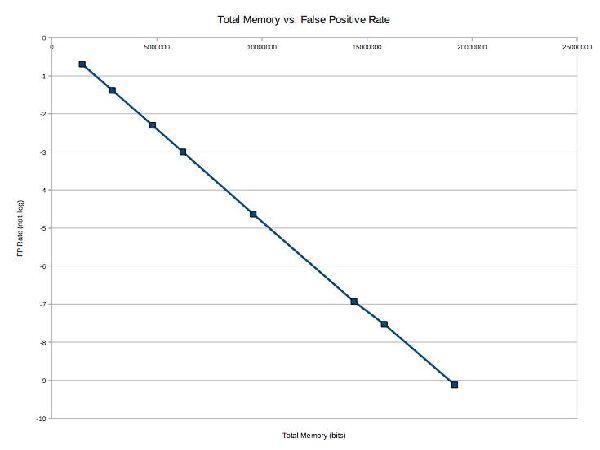
\includegraphics[width=5in]{figures/f2b}}
\caption{Bloom filters scale well.}
\end{figure}

\begin{figure}
\center{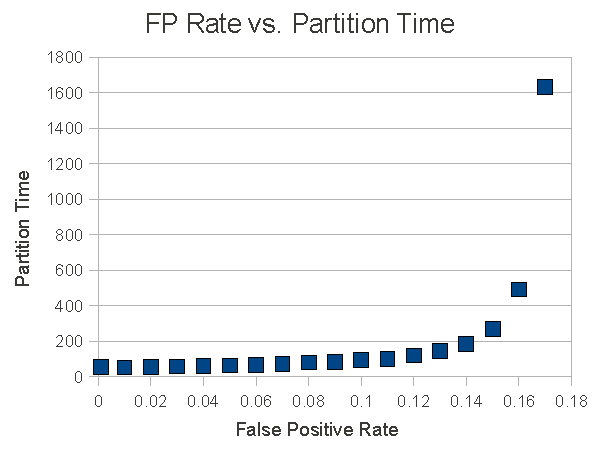
\includegraphics[width=5in]{figures/f3d}}
\caption{Computation required to partition graphs grows with false positive
rate.  CTB: good to know, but I think this figure can go away; it's implied
by everything else.}
\end{figure}

\begin{figure}
\center{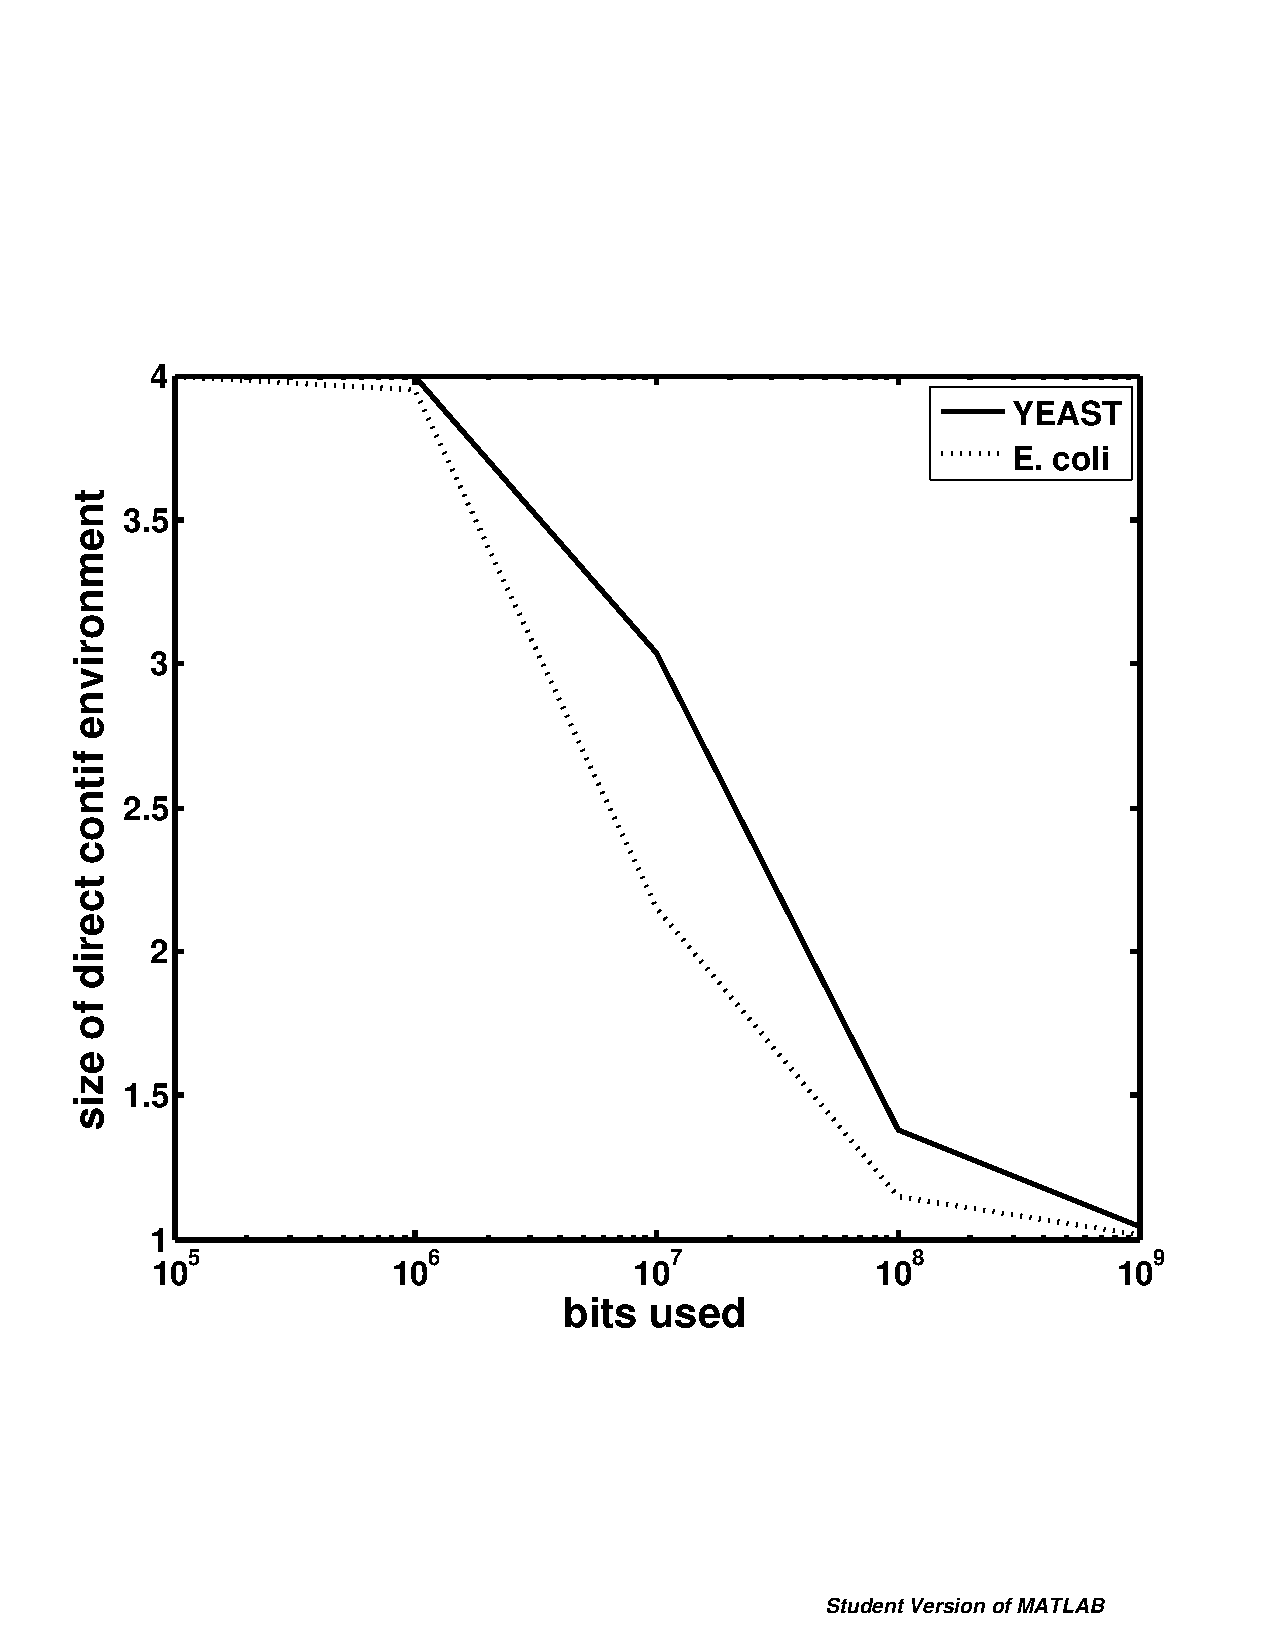
\includegraphics[width=5in]{contigEnvironment}}
\caption{Number of false connections introduced by inexact k-mer storage.
k = ??}
\end{figure}

\begin{figure}
\center{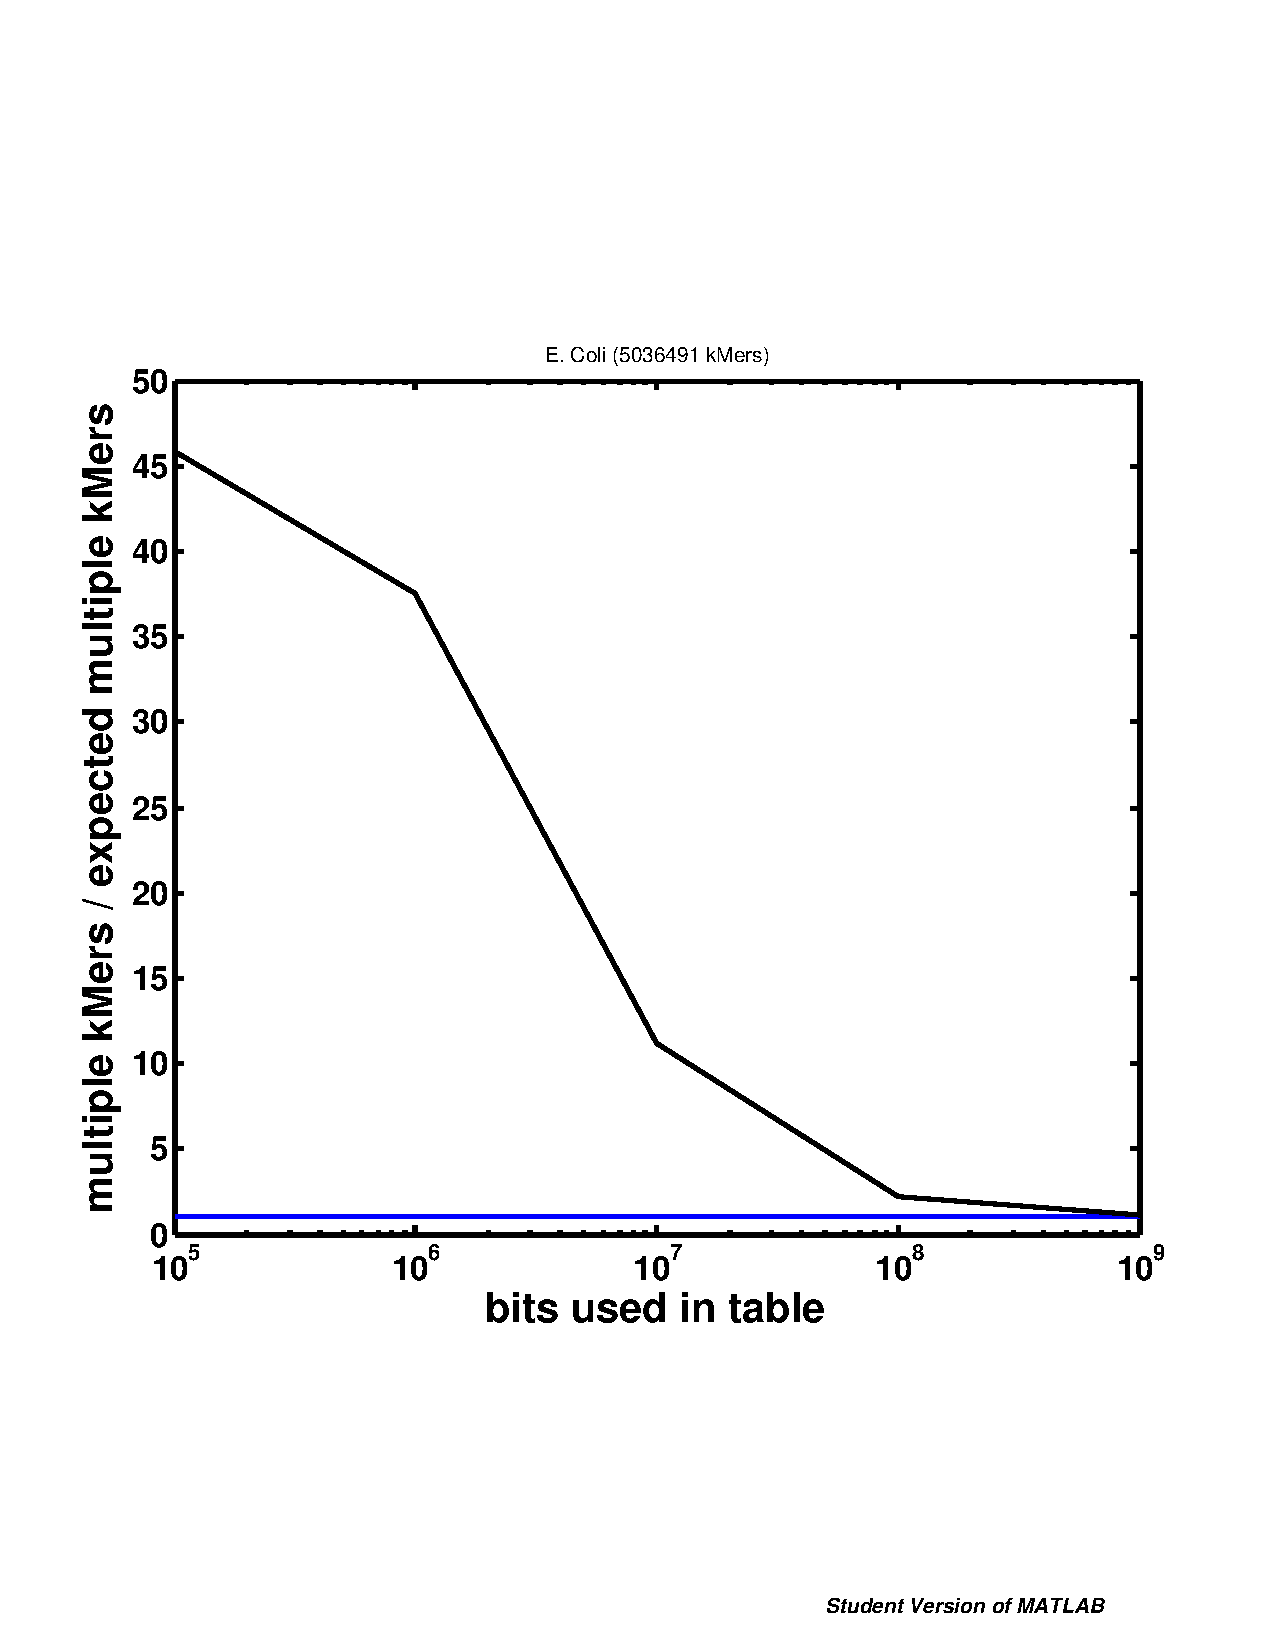
\includegraphics[width=5in]{fractionOfFoundDoubleHitsECOLI}}
\caption{The difference between exact and inexact kmer storage for the
ecoli genome. k = ??}
\end{figure}

\begin{figure}
\center{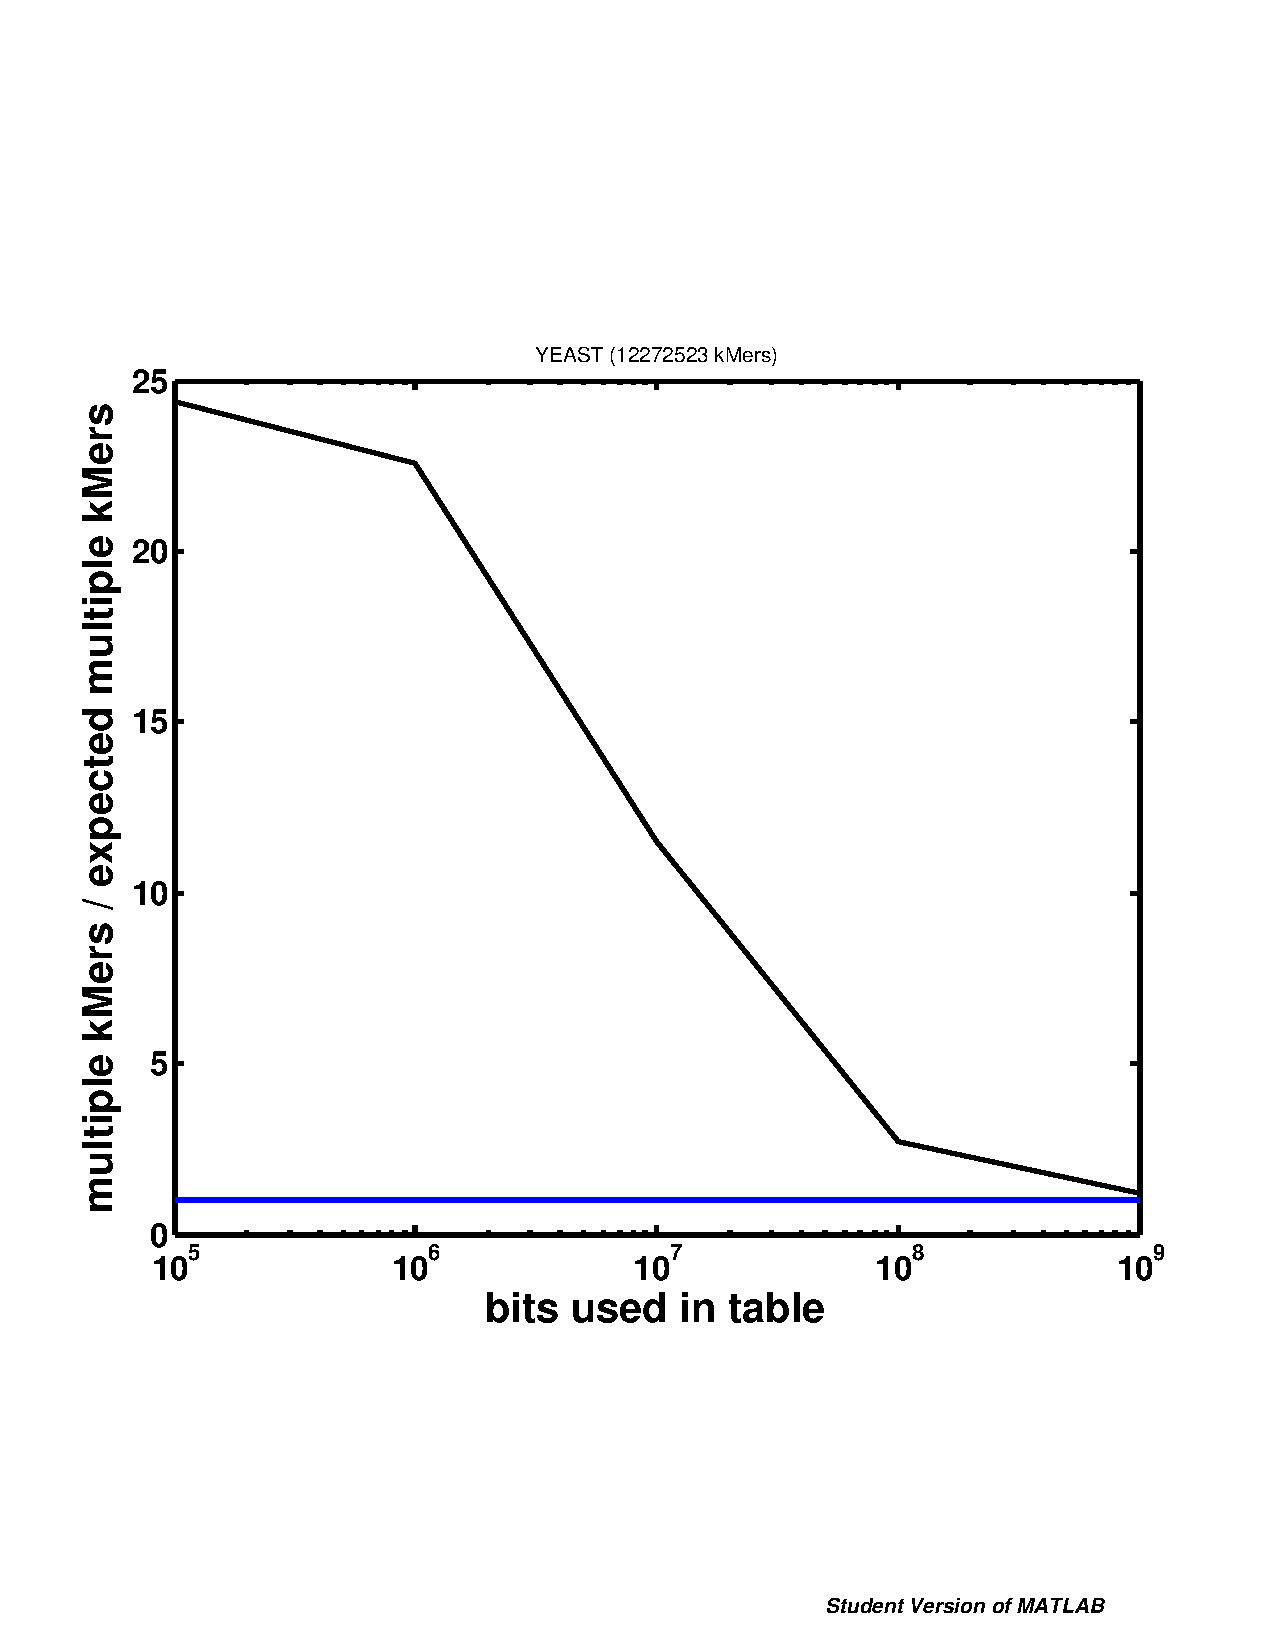
\includegraphics[width=5in]{fractionOfFoundDoubleHitsYEAST}}
\caption{The difference between exact and inexact kmer storage for the
yeast genome. k = ??}
\end{figure}

\end{document}


